% -*- TeX:UTF-8 -*-
%%
%% KAIST 학위논문양식 LaTeX용 (ver 0.5) 예시
%%
%% @version 0.4
%% @author  채승병 Chae,Seungbyung (mailto:chess@kaist.ac.kr)
%% @date    2004. 11. 12.
%%
%% @requirement
%% teTeX, fpTeX, teTeX 등의 LaTeX2e 배포판
%% + 은광희 님의 HLaTeX 0.991 이상 버젼 또는 홍석호 님의 HPACK 1.0
%% : 설치에 대한 자세한 정보는 http://www.ktug.or.kr을 참조바랍니다.
%%
%% @note
%% 기존에 널리 쓰여오던 차재춘 님의 학위논문양식 클래스 파일의 형식을
%% 따르지 않고 전면적으로 다시 작성하였습니다. 논문 정보 입력부분에서
%% 과거 양식과 다른 부분이 많으니 아래 예시에 맞춰 바꿔주십시오.
%%
%%
%% @acknowledgement
%% 본 예시 논문은 물리학과 박사과정 김용현 님의 호의로 제공되었습니다.
%%
%% -------------------------------------------------------------------
%% @information
%% 이 예제 파일은 hangul-ucs를 사용합니다. UTF-8 입력 인코딩으로
%% 작성되었습니다. hlatex의 hfont는 이용하지 않습니다. --2006/02/11
%% 본 템플릿은 전산학부 김민혁 교수에의해서 버그 수정되었습니다. -- 2016/11/25

% @class kaist.cls
% @options [default: doctor, korean, final]
% - doctor: 박사과정 | master : 석사과정
% - korean: 한글논문 | english: 영문논문
% - final : 최종판   | draft  : 시험판
% - pdfdoc : 선택하지 않으면 북마크와 colorlink를 만들지 않습니다.


\documentclass[master,english,final]{kaist-ucs}


% If you want make pdf document (include bookmark, colorlink)
%\documentclass[doctor,english,final,pdfdoc]{kaist-ucs}

% kaist.cls 에서는 기본으로 dhucs, ifpdf, graphicx 패키지가 로드됩니다.
% 추가로 필요한 패키지가 있다면 주석을 풀고 적어넣으십시오,
%\usepackage{...}
\usepackage{comment}
\usepackage{subcaption}
\usepackage{algorithm}
\usepackage{algpseudocode}
\usepackage{tabularx}
\usepackage{amsmath}
\usepackage{caption}
\usepackage{float}

\makeatletter
\providecommand{\bstctlcite}[1]{%
  \@bsphack
  \@for\@citeb:=#1\do{%
    \edef\@citeb{\expandafter\@firstofone\@citeb}%
    \if@filesw
      \immediate\write\@auxout{\string\citation{\@citeb}}%
    \fi
  }%
  \@esphack
}
\makeatother

% @command title 논문 제목(title of thesis)
% @options [default: (none)]
% - korean: 한글제목(korean title) | english: 영문제목(english title)
\title[korean] {RL-SchedExt: 커널 내 신경망 추론 기반\linebreak 긴급도 인식 CPU 스케줄링}
\title[english]{RL-SchedExt: Urgency-Aware CPU Scheduling\linebreak with In-Kernel Neural Inference}

% @note 표지에 출력되는 제목을 강제로 줄바꿈하려면 \linebreak 을 삽입.
%       \\ 나 \newline 등을 사용하면 안됩니다. (아래는 예시)
%
%\title[korean]{탄소 나노튜브의 물리적 특성에 대한\linebreak 이론 연구}
%\title[english]{Theoretical study on physical properties of\linebreak
%                carbon nanotubes}
%
% If you want to begin a new line in cover, use \linebreak .
% See examples above.
%


% @command author 저자 이름
% @param   family_name, given_name 성, 이름을 구분해서 입력
% @options [default: (none)]
% - korean: 한글이름 | chinese: 한문이름 | english: 영문이름
% 한문 이름이 없다면 빈 칸으로 두셔도 됩니다.
%
%
% If you are a foreigner , write your name in korean or your korean name.
% If you can't write native character, you can make the chinese blank empty 
% Write as follow
% \author[korean]{family name in korean}{given name in korean}
% \author[chinese]{family name in your native language}{given name in your native language}
% \author[english]{family name in english}{given name in english}
%
\author[korean]{이}{재 원}
\author[korean2]{이}{재원}    %이름을 붙여 써 주시기 바랍니다.
\author[chinese]{李}{載遠}
\author[english]{Lee}{Jaewon}

% @command advisor 지도교수 이름 (복수가능)
% @usage   \advisor[options]{...한글이름...}{...영문이름...}{signed|nosign}
% @options [default: major]
% - major: 주 지도교수  | coopr: 공동 지도교수
\advisor[major]{원 유 집}{Youjip Won}{signed}
\advisor[major2]{원유집}{Youjip Won}{signed}    %한글 성과 한글 이름을 모두 붙여 써 주시기 바랍니다.
\advisorinfo{Professor of Graduate School of System Architect} %제출승인서에 들어가는 교수님 정보, advisor's information 
%\advisor[coopr]{김 동 준}{Dongjun Kim}{nosign}
%\advisor[coopr2]{김동준}{Dongjun Kim}{nosign}    %한글 성과 한글 이름을 모두 붙여 써 주시기 바랍니다.
%
% 지도교수 한글이름은 입력하지 않아도 됩니다.
% You may not input advisor's korean name
% like this \advisor[major]{}{Chang, Kee Joo}{signed}
%


% @command department {학과이름}{학위종류} - 아래 규칙에 따라 코드를 입력
% @command department {department code}{degree field}
%
% department code
% 2. 석박사학위논문 작성 및 제출요령 4쪽 ~ 5쪽 참고
% 또는 kaist-ucs.cls 의 % @command department 참고

% science: 이학 | engineering: 공학 | business : 경영학
% 박사논문의 경우는 학위종류를 입력하지 않아도 됩니다.
% If you write Ph.D. dissertation, you cannot input degree field.
% The third parameter : a | b | c
% a: 소속된 학과만 쓰는 옵션 (학과에만 소속되어 있는 경우에는 무조건 a를 선택해야 함)
% b: 학과 아래의, 프로그램이나 학제전공에 소속되어 있을 경우에 학과와 프로그램을 함께 쓰는 옵션
% c: 학과 아래의, 프로그램이나 학제전공에 소속되어 있을 경우에 학과를 쓰지 않고 프로그램이나 학제전공의 이름만 쓰는 옵션 
% 
% a: it represents only the name of department. (if you aren't in the program under the department, must choose a)
% b: it represents the names of department and the program that is under the department (consider this when you are in the program not only department)
% c: it represents only the name of program that is under the department (consider this when you are in the program not only department)
\department{SA}{engineering}{a}

% @command referee 심사위원 (석사과정 3인, 박사과정 5인)
\referee[1]{원 유 집}
\referee[2]{권 영 진}
\referee[3]{신 인 식}
% \referee[5] {Barack Obama}
% Of course english name is available

% @command approvaldate 지도교수논문승인일
% @param   year,month,day 연,월,일 순으로 입력
\approvaldate{2027}{1}{1}

% @command refereedate 심사위원논문심사일
% @param   year,month,day 연,월,일 순으로 입력
\refereedate{2027}{1}{1}

% @command gradyear 졸업년도
\gradyear{2027}

% 본문 시작
\begin{document}
\bstctlcite{IEEEexample:BSTcontrol}

    % 앞표지, 속표지, 학위논문 제출승인서, 학위논문 심사완료 검인서는
    % 클래스 옵션을 final로 지정해주면 자동으로 생성되며,
    % 반대로 옵션을 draft로 지정해주면 생성되지 않습니다.

    % 논문 서지, 초록, 핵심 낱말, 영문 초록, 영어 핵심 낱말 (Information of thesis, abstract in korean, keywords in korean, abstract in english, keywords in english)
   \thesisinfo
   %% Letters of abstract in korean must be less than 500 and words of abstract in english must be less than 300.
   %% Number of keywords must be less than 6.
   %% Don't write english letters in the abstract in korean.
    \begin{summary}      
    Modern Android 시스템에서 multimedia application의 서비스 품질은 개별 request가 요구된 시간 내에 완료되는지에 크게 영향을 받는다. 그러나 기존 CPU Scheduler는 application-level deadline을 직접 관측할 수 없으며, 주로 공정성(Fairness)을 기반으로 task의 실행 순서를 결정한다. 본 논문에서는 이러한 문제를 해결하기 위해 강화학습(Reinforcement Learning, RL)과 커널 내 신경망 추론(In-Kernel Neural Inference)을 활용한 긴급도 인식(Urgency-aware) CPU Scheduling Framework인 RL-SchedExt를 제안한다.
    
    RL-SchedExt는 다양한 task의 실행 특성, CPU 경쟁(Contention) 및 task 간 의존성(Dependency)을 모사하는 Scheduling Simulator와의 상호작용을 통해 문맥 의존적(Context-dependent) Scheduling Policy를 학습한다. 학습된 Policy는 교사-학생 지식 증류(Teacher-Student Knowledge Distillation)와 8-bit 양자화(Quantization)를 통해 경량 신경망(Neural Network)으로 변환된다. Runtime에서는 Neural Network가 Kernel에서 관측 가능한 State를 기반으로 각 task의 상대적인 스케줄링 긴급도(Scheduling Urgency)를 추론하고, 실행 가능한(Runnable) task의 가상 실행 시간(Vruntime)에 Learned Vruntime Adjustment를 반영하여 긴급도 인식 가상 실행 시간(Urgency-aware Vruntime)을 계산한다. 기존 Vruntime Accounting 값은 변경하지 않으며, 계산된 값은 eBPF 기반 sched\_ext Framework에서 Task Selection에 사용된다.
    
    Android 15가 탑재된 Google Pixel 9 Pro XL에서 평가한 결과, RL-SchedExt는 기존 Completely Fair Scheduler(CFS) 대비 Deadline Miss를 19.4–26.8\%, 총 Deadline 초과량(Total Deadline Overrun)을 4.5–19.3\% 감소시켰다. 또한 동일한 State와 Action을 사용하는 조건에서 신경망 기반 정책(Neural Policy)은 선형 정책(Linear Policy)보다 높은 Deadline 준수율(Deadline Compliance)을 달성하였다. 실제 Android Gaming Workload에서는 평균 FPS를 11.9\% 향상시키는 동시에 Frame Interval의 꼬리 지연 시간(Tail Latency)을 감소시켰다. 이러한 결과는 경량 비선형 스케줄링 정책(Nonlinear Scheduling Policy)이 Runtime에서 명시적인 Deadline 정보 없이도 application-level Deadline Compliance를 향상시키는 데 효과적임을 보여준다.

    \end{summary}
   
    \begin{Korkeyword}
    강화학습, 중앙처리장치 스케줄링, 긴급도 인식 스케줄링,
    커널 내 신경망 추론, 지식 증류
    \end{Korkeyword}

    \clearpage
    \begin{abstract}
    The quality of service of multimedia applications on modern Android systems depends on the timely completion of individual requests. However, conventional CPU schedulers determine task execution order primarily based on fairness, without direct knowledge of application-level deadlines. This dissertation presents RL-SchedExt, an urgency-aware CPU scheduling framework that leverages reinforcement learning and in-kernel neural inference.
    
    RL-SchedExt learns a context-dependent scheduling policy through interaction with a scheduling simulator that models diverse task execution patterns, CPU contention, and task dependencies. The learned policy is transferred to a lightweight neural network through teacher–student knowledge distillation and 8-bit quantization. During runtime, the neural network infers relative task urgency from kernel-observable states and computes an urgency-aware virtual runtime for each runnable task by applying a learned adjustment to its virtual runtime. The underlying virtual runtime accounting remains unchanged, and the computed value is used for task selection through the eBPF-based sched\_ext framework.
    
    Evaluation on a Google Pixel 9 Pro XL running Android 15 demonstrates that RL-SchedExt reduces deadline misses by 19.4–26.8\% and total deadline overrun by 4.5–19.3\% compared with the Completely Fair Scheduler (CFS). Furthermore, the neural policy achieves better deadline compliance than its linear counterpart under identical state and action representations. In a real-world Android gaming workload, RL-SchedExt improves average FPS by 11.9\% while reducing frame interval tail latency. These results demonstrate the effectiveness of lightweight nonlinear scheduling policies in improving application-level deadline compliance without explicit deadline information during runtime.
    \end{abstract} 
     
    \begin{Engkeyword}
    Reinforcement Learning, CPU Scheduling,
    Urgency-Aware Scheduling, In-Kernel Neural Inference,
    Knowledge Distillation
    \end{Engkeyword}
   

    \addtocounter{pagemarker}{1}                 % 백색별지분을 고려
    \newpage 
  


    % % 목차 (Table of Contents) 생성
    % \tableofcontents

    % % 표목차 (List of Tables) 생성
    % \listoftables

    % % 그림목차 (List of Figures) 생성
    % \listoffigures

    % 위의 세 종류의 목차는 한꺼번에 다음 명령으로 생성할 수도 있습니다.
    \makecontents

%% 이하의 본문은 LaTeX 표준 클래스 report 양식에 준하여 작성하시면 됩니다.
%% 하지만 part는 사용하지 못하도록 제거하였으므로, chapter가 문서 내의
%% 최상위 분류 단위가 됩니다.
%% You cannot use 'part'

\chapter{Introduction}
{\color{blue} 1차 수정 완료 v0.1}

{\color{blue} CFS가 deadline urgency task 대신 다른 task 수행하는 사례 첨부하면 좋음}
\section{Motivation and Challenges}
Modern Android 시스템에서는 interactive applications, multimedia processing,백그라운드 연산 등 다양한 특성을 가진 Workload가 제한된 CPU 자원을 공유한다.
특히 게임과 영상 스트리밍 등 멀티미디어 application의 활용이 확대되면서, 사용자 경험(User Experience)은 multimedia processing에 관련된 개별 request가 요구된 시간 안에 완료되는지에 더욱 민감해지고 있다.
일부 request가 deadline을 초과하거나 완료 시간이 크게 지연되면, frame drop, 화면 끊김(Stuttering) 등이 발생할 수 있다.
따라서 deadline compliance와 tail latency는 Android application의 responsiveness와 서비스 품질을 평가하는 중요한 성능 지표이다.

Linux 6.6 이전의 Completely Fair Scheduler(CFS)는 각 task의 Virtual Runtime(Vruntime)을 기반으로 task ordering을 결정하여 fairness를 유지한다. 
Linux 6.6부터 도입된 Earliest Eligible Virtual deadline First(EEVDF)는 Virtual deadline을 이용하여 task ordering을 개선하였지만, 이 값은 application request의 실제 deadline이나 urgency를 나타내지는 않는다. 
두 scheduler는 모두 fairness를 중심으로 task ordering을 결정하며, 개별 application request의 deadline이나 task 간 dependency가 request completion time에 미치는 영향을 직접적인 scheduling 기준으로 사용하지 않는다. 
Nice value와 Cgroup을 통해 task 및 task Group의 상대적인 Scheduling Weight를 조절할 수 있지만, 이러한 설정만으로는 유사한 priority를 가진 task사이에서 동적으로 변화하는 deadline urgency를 구분하기 어렵다. 
따라서 기존 Scheduler의 fairness를 활용하면서도 scheduling context에 따라 task ordering을 조정할 필요가 있다.

Task의 scheduling urgency는 해당 task의 속성만으로 결정되지 않는다.
예를 들어 deadline이 임박한 request를 처리하는 task를 먼저 실행하는 것이 유리한 경우가 있는 반면, 다른 task의 진행을 막고 있는 Lock Holder나 선행 task를 우선 실행하는 것이 전체 request의 deadline miss를 줄이는 상황도 존재한다.
또한 CPU contention과 Wakeup pattern이 변화하면 동일한 task의 상대적인 scheduling urgency도 달라질 수 있다.
Reinforcement Learning(RL)은 고정된 priority rule 대신 scheduling decision action 이후의 request latency와 deadline miss에 미치는 영향을 reward로 학습하여, 이러한 context-dependent task ordering에 대응할 수 있다.

이 문제를 해결하는 데에는 두 가지 기술적 어려움이 존재한다.

\begin{itemize}
    \item Kernel Scheduler는 개별 application request의 실제
    deadline이나 남은 CPU Demand를 일반적으로 직접 관측할 수 없다.
    따라서 Scheduling Policy는 Virtual Runtime, CPU 사용 이력,
    Runnable Waiting Time, Wakeup History 등 Kernel에서 관측
    가능한 정보로부터 task의 상대적 중요도를 추론해야 한다.

    \item Context-dependent 판단을 복잡한 Machine Learning
    Model로 수행할 경우 Scheduling Critical Path에 추가적인
    연산 비용이 발생한다. 특히 짧은 간격으로 task Selection이 반복되는 환경에서는
    추론 비용 자체가 Scheduling Latency를 증가시켜 
    학습된 정책의 성능 이득을 상쇄할 수 있다.

\end{itemize}

\section{RL-SchedExt Overview}

본 논문에서는 이러한 문제를 해결하기 위해 Offline Reinforcement Learning으로 학습한 task ordering policy를 Android Kernel에서 실행하는 CPU scheduling framework인 RL-SchedExt를 제안한다.
핵심 아이디어는 RL을 통해 scheduling context에 따른 Learned Vruntime Adjustment를 학습하고, 이를 CFS 기반 Vruntime에 반영하여 각 task의 Urgency-aware Vruntime을 계산하는 것이다. 
Scheduler는 Urgency-aware Vruntime을 기준으로 task ordering을 결정함으로써, 기존 fairness 기반 Scheduling에 각 task의 deadline Urgency를 고려한 실행 순서를 반영한다.

RL Teacher의 학습에는 가상 시간 기반 scheduling simulator를 사용한다.
Simulator는 task arrival, CPU demand, wakeup, blocking, dependency와 scheduling decision에 따른 vruntime 변화를 모사한다.
다양한 실행 특성을 가진 task를 조합하여 scheduling context를 생성하고, RL Teacher는 simulator와 상호작용하면서 이후의 request latency와 deadline miss에 기반한 reward를 통해 policy를 학습한다.
이 과정은 실제 Android 배포 이전에 수행되는 simulator-based offline training이다.

학습된 Teacher policy를 Android Kernel에 직접 적용하는 대신, RL-SchedExt는 Teacher--Student Distillation을 이용하여 경량 Neural Student Policy를 생성한다.
Student는 각 Runnable task의 실행 이력과 CPU의 Global State로부터 구성한 57차원 입력을 사용하며, task Encoder와 Set-context Aggregation을 통해 현재 경쟁 중인 task들의 상대적 특성을 함께 반영한다.
이러한 구조는 경쟁하는 task들의 상태에 따라 각 task의 상대적인 순서를 달리 결정할 수 있도록 한다.
Teacher training과 distillation은 모두 Offline에서 수행하며, Android에서는 경량 student policy만 실행한다.

Android runtime에서는 native kernel code가 Scheduling History를 수집하여 task별 57차원 state를 생성한다.
Student는 각 task의 State를 입력받아 Urgency-aware adjustment를 계산한다.
Native Kernel에서 계산된 Learned Vruntime Adjustment는 각 Task의 CFS 기반 Vruntime에 반영되어 Urgency-aware Vruntime을 생성한다. 이후 sched\_ext의 eBPF 프로그램은 Urgency-aware Vruntime을 기준으로 task ordering을 수행한다.
이러한 방식은 CFS의 fairness 기반 Scheduling 기준을 활용하면서도, 실행 시점의 Workload 특성과 추론된 task urgency에 따라 실행 순서를 조정할 수 있도록 한다.

\section{Evaluation and Contributions}
RL-SchedExt를 Google Pixel 9 Pro XL의 실제 Android 15 환경에서 평가하였다.
평가 대상은 Linux 6.1 기반 kernel로, 해당 환경의 기본 fair scheduler인
CFS를 baseline으로 사용하였다.
EEVDF는 이후 Linux 버전에서 도입된 방식이므로 본 실험의 baseline에는 포함하지 않았다.
Microbenchmark에서는 짧고 빈번한 Wakeup과 긴 CPU Burst가 경쟁하는 상황, Lock을 통해 task 간 Dependency가 발생하는 상황, 그리고 실행 도중 Workload의 특성이 변화하는 상황을 포함한 세 가지 Workload를 평가하였다.
그 결과 Neural Student는 CFS 대비 deadline miss를 19.4--26.8\%, Total deadline Overrun을 4.5--19.3\% 감소시켰다.
request Completion Latency p99는 일부 Workload에서 소폭 증가하였다.
특히 \textit{Mixed CPU Bursts}에서는 Deadline Budget이 4\,ms 미만인 Request의
p99가 25.3\% 감소한 반면, 8\,ms 이상인 Request의 p99는 3.7\% 증가하였다.
이는 짧은 Deadline 제약을 가진 Request의 Latency를 줄이는 과정에서
상대적으로 긴 Deadline 제약을 가진 Request의 Latency가 증가할 수 있음을
보여준다.

실제 application 수준의 성능을 평가하기 위해 Android 게임 \textit{Mindustry}를 이용한 Macrobenchmark도 수행하였다.
동일한 게임 시나리오에서 RL-SchedExt는 CFS 대비 average FPS를 11.9\% 향상시켰다.
또한 frame interval p99는 86\,ms에서 66\,ms로 감소하여 23.3\% 개선되었으며,
frame interval p50과 p95는 동일하게 유지되었다.
이는 일반적인 frame 출력 간격을 유지하면서 긴 출력 지연을 줄여,
평가한 게임 workload에서 frame pacing을 개선했음을 보여준다.

본 논문의 주요 기여는 다음과 같다.

\begin{itemize}
    \item Learning-based task ordering:
    fairness 기반 task ordering과 application deadline Compliance
    사이의 불일치를 Scheduling 문제로 정의하고,
    다양한 task 실행 특성과 Dependency가 포함된 Simulator에서
    장기적인 성능을 고려한 Urgency-aware Vruntime Adjustment
    Policy를 학습하는 방법을 제시한다.

    \item Deployable Nonlinear Scheduling Policy:
    Offline Teacher--Student Distillation을 통해
    Runnable task 간 Context를 반영하는 경량 Neural Policy를
    구성하고, 이를 Native Kernel Inference와 eBPF 기반
    task Selection으로 통합한다.

    \item Real-device Evaluation and Policy Analysis:
    실제 Android에서 CFS 및 Linear Student와 비교하여
    deadline miss와 deadline Overrun의 개선을 정량적으로
    평가하고, 잔여 deadline에 따른 Urgency-aware Adjustment
    분석을 통해 학습된 task ordering의 특성을 조사한다.
\end{itemize}

\chapter{Background}
% {\color{blue} 초안 작성 v0.0}

% {\color{blue} subsection에 대한 고민 필요}

% {\color{blue} A.비교군 / B.평가지표설명 / C.RL구조 / D.Sched\_Ext로 구성. }

\section{Fair Scheduling and Virtual Runtime}

Linux의 Completely Fair Scheduler(CFS)는 각 Task의 Scheduling
Weight에 비례하여 CPU 자원을 분배하는 것을 목적으로 한다.
CFS는 실제 CPU Execution Time을 Scheduling Weight에 따라
정규화한 Virtual Runtime(Vruntime)을 이용하여 각 Task의 상대적인
CPU 사용량을 관리한다.
Task $i$가 $\Delta t_i$만큼 CPU를 사용하였을 때 Vruntime의
증가량은 다음과 같이 표현할 수 있다.

\begin{equation}
    V_i(t+\Delta t_i)-V_i(t) = \Delta t_i \frac{w_0}{w_i},
\end{equation}

여기서 $w_i$는 Task $i$의 Scheduling Weight이며,
$w_0$는 nice 0에 해당하는 기준 Scheduling Weight이다.
높은 Scheduling Weight를 가진 Task는 동일한 CPU Execution Time에 대해
Vruntime이 상대적으로 적게 증가하므로 더 많은 CPU 실행 기회를
확보할 수 있다.
CFS는 동일 Runqueue 내에서 Vruntime이 작은 Scheduling Entity를
우선적으로 선택함으로써 장기적인 CPU 자원 분배의 Fairness를
유지한다.

Linux 6.6부터 도입된 Earliest Eligible Virtual Deadline
First(EEVDF)는 기존 Vruntime에 기반한 CPU 사용량 관리에
Eligibility와 Virtual Deadline이라는 개념을 추가한다.
EEVDF는 할당받아야 할 CPU 자원보다 적은 자원을 사용한
Eligible Task 중 가장 이른 Virtual Deadline을 가진 Task를
우선적으로 선택한다.
그러나 Virtual Deadline은 Scheduling Weight와 요청된
CPU 실행 구간에 기반하여 계산되는 가상 시간상의 값으로,
Application Request의 실제 Deadline과는 구분된다.
따라서 CFS와 EEVDF에서 정의하는 실행 우선순위는
Application Request의 시간적 제약과 반드시 일치하지 않는다.


\section{Request-Level Deadlines and Task Dependencies}

Task는 CPU Scheduler가 관리하는 실행 단위이며,
Request는 Application이 완료해야 하는 작업 단위이다.
Workload는 이러한 Task와 Request 및 이들의 실행 패턴과
의존 관계를 포함하는 전체 작업 구성을 의미한다.
하나의 Task는 여러 Request를 반복적으로 처리할 수 있으며,
반대로 하나의 Request가 완료되기 위해 여러 Task의 실행과
Synchronization이 필요할 수도 있다.
예를 들어 Multimedia Application의 Frame Processing은
여러 Task의 연산, Wakeup, Blocking 및 Synchronization을
포함할 수 있다.

Request $j$의 Arrival Time, Completion Time 및
Absolute Deadline을 각각 $a_j$, $c_j$, $d_j$라고 정의한다.
Deadline Budget은 Request의 Arrival Time부터 Absolute Deadline까지
허용된 전체 시간이며, Remaining Deadline은 현재 시각 $t$에서
Absolute Deadline까지 남은 시간을 의미한다.

\begin{equation}
    \mathrm{Deadline\ Budget}_j = d_j-a_j,\qquad
    \mathrm{Remaining\ Deadline}_j(t) = d_j-t.
    \label{eq:deadline_times}
\end{equation}

Deadline Budget은 Request마다 정해지는 값인 반면,
Remaining Deadline은 시간에 따라 감소하며 Deadline이 지나면 음수가 된다.
이와 달리 Remaining CPU Demand는 Request를 완료하기 위해
추가로 필요한 CPU 실행 시간을 의미한다.

Request Completion Latency($L_j$), Deadline Miss($M_j$),
Deadline Overrun($O_j$)은 다음과 같이 표현할 수 있다.

\begin{equation}
    L_j = c_j - a_j,\qquad M_j = \mathbf{1}[c_j > d_j],\qquad O_j = \max(0, c_j - d_j).
\end{equation}

Deadline Miss는 Request가 시간적 제약을 충족하지 못하였는지를
나타내며, Deadline Overrun은 해당 제약을 얼마나 초과하였는지를
나타낸다.
Deadline Miss만을 최소화하는 정책은 이미 Deadline을 초과한
Request의 실행을 지연시키더라도 추가적인 불이익을 받지 않을 수
있으므로, Request Completion Latency와 Deadline Overrun을
함께 고려할 필요가 있다.

본 논문에서 Scheduling Urgency는 Request의 Deadline Compliance를
향상시키기 위해 해당 Task를 우선 실행할 필요성을 의미한다.
Scheduling Priority는 Scheduling Policy가 결정하는 상대적인 실행
우선순위를 의미하므로 Scheduling Urgency와 구분된다.
Request의 Deadline과 해당 Request에 관여하는 Task의
Scheduling Urgency는 반드시 일치하지 않는다.
예를 들어 Remaining Deadline이 짧은 Request를 처리하는 Task가
Lock을 기다리고 있다면, 해당 Task를 직접 실행하는 대신
Lock Holder를 먼저 실행하는 것이 Request Completion을
앞당길 수 있다.
따라서 Task의 Scheduling Urgency는 개별 Request의
Remaining Deadline뿐만 아니라 Remaining CPU Demand, Task 간 Dependency 및
현재의 CPU Contention에 의해서도 결정된다.


\section{Extensible Scheduling with sched\_ext}

Linux 6.12에 도입된 sched\_ext는 eBPF Scheduling Program을 통해
사용자 정의 CPU Scheduling Policy를 구현할 수 있도록
지원하는 Scheduler Class이다.
sched\_ext는 CPU Selection, Task Enqueue 및 Dispatch 등의
Scheduling Operation에 대한 Interface를 제공한다.

sched\_ext는 Dispatch Queue(DSQ)를 이용하여 eBPF Scheduling Program과
Kernel Scheduler Core 사이에서 Runnable Task를 관리한다.
DSQ는 FIFO 또는 Virtual Time 기반의 Priority Queue로
동작할 수 있으며, 이를 통해 사용자 정의 Scheduling Metric에
따른 Task Ordering을 구현할 수 있다.
본 논문에서 Task Ordering은 Task 간 상대적인 실행 순서를,
Task Selection은 다음 실행할 Task를 선택하는 행위를,
Task Dispatch는 선택된 Task를 Kernel의 실제 실행 경로에
반영하는 과정을 의미한다. Scheduling Decision은 이러한 실행 대상에
대한 Scheduling Policy의 의사결정을 의미한다.

그러나 CPU Scheduling은 빈번하게 수행되는 Kernel Critical
Path에 해당하므로, Scheduling Policy의 추가적인 연산 비용은
전체 시스템의 성능에 직접적인 영향을 미칠 수 있다.
또한 eBPF Scheduling Program은 Verifier를 통해 메모리 접근의 안전성과
프로그램 실행의 유효성을 검증받아야 하므로, 복잡한 연산을
포함하는 Machine Learning Model을 구현하는 데 제약이 존재한다.

따라서 학습 기반 Scheduling Policy를 Kernel에 적용하기
위해서는 Model의 표현력뿐만 아니라 Inference Cost와
Scheduling Decision의 실행 비용을 함께 고려해야 한다.


\section{Learning-based Scheduling Techniques}

\paragraph{Reinforcement Learning (RL).}
RL은 Agent가 Environment와 상호작용하면서 State에 따른
Action을 결정하고, 그 결과로 주어지는 Reward를 통해
Policy를 학습하는 방법이다.
RL의 목적은 개별 Action의 즉각적인 Reward뿐만 아니라
이후의 누적 Reward를 최대화하는 Policy를 학습하는 것이다.
CPU Scheduling에서는 현재의 Task Selection이 이후 Task의
Runnable Waiting Time, Wakeup 및 Request Completion에 연쇄적으로 영향을
미치므로, RL을 통해 연속적인 Scheduling Decision의
장기적인 성능 영향을 고려할 수 있다.

\paragraph{DeepSets.}
DeepSets는 원소의 개수가 가변적이고 입력 순서에 의미가
없는 집합 형태의 데이터를 처리하기 위한 Neural Network
Architecture이다.
각 원소를 공유된 Encoder $\phi$를 통해 개별적으로
Encoding하고, 이를 순서에 독립적인 Aggregation
Operation을 통해 하나의 Context로 표현한다.

\begin{equation}
    z = \rho \left( \sum_{i=1}^{N} \phi(x_i) \right),
\end{equation}

여기서 $x_i$는 집합의 개별 원소이며, $\rho$는
Aggregation된 Feature를 변환하는 함수이다.
이러한 구조는 입력 원소의 개수와 순서가 달라지더라도
집합 전체의 특성을 고정된 차원의 Representation으로
표현할 수 있다.
CPU Scheduling에서는 경쟁하는 Runnable Task의 수가
동적으로 변화하므로, DeepSets를 통해 개별 Task의
특성과 경쟁 Task들의 Context를 함께 고려할 수 있다.

\paragraph{Teacher--Student Knowledge Distillation (KD).}
Teacher--Student Knowledge Distillation은 높은 표현력을 가진 Teacher
Model의 학습된 Knowledge를 상대적으로 경량화된
Student Model에 전달하는 방법이다.
Student는 Teacher의 Output 또는 Policy Distribution을
학습 목표로 사용하여 Teacher의 동작을 근사한다.
이를 통해 Training 단계에서는 높은 연산 비용을 요구하는
복잡한 Model을 활용하고, Deployment 단계에서는 제한된
연산 자원에 적합한 경량 Model을 실행할 수 있다.
이러한 Training과 Inference의 분리는 실행 비용에
민감한 CPU Scheduling 환경에서 학습 기반 Policy를
적용하는 데 유용하다.


\chapter{System Design}
% {\color{blue} 정돈되어있지 않아 정리 및 단어 통일화필요}

% {\color{blue} workload generate figure 필요한가? }

\section{Design Overview}
\label{sec:design_overview}

Figure~\ref{fig:system_overview}는 RL-SchedExt의 전체 System Architecture를 나타낸다.
RL-SchedExt는 Scheduling Policy를 학습하는 Offline Learning
단계와 학습된 Policy를 실제 CPU Scheduling에 적용하는
Runtime Inference 단계로 구성된다.
Offline Learning은 Linux Server에서 수행되며,
Runtime Inference는 Android Kernel 내부에서 수행된다.
이러한 구조는 Deadline 기반의 Reward를 확보하기 어려운
실제 Kernel 환경에서 학습을 수행할 필요 없이,
학습된 Scheduling Policy를 적용할 수 있도록 한다.

\begin{figure}[H]
    \centering
    \IfFileExists{Figures/System_overview.png}{%
        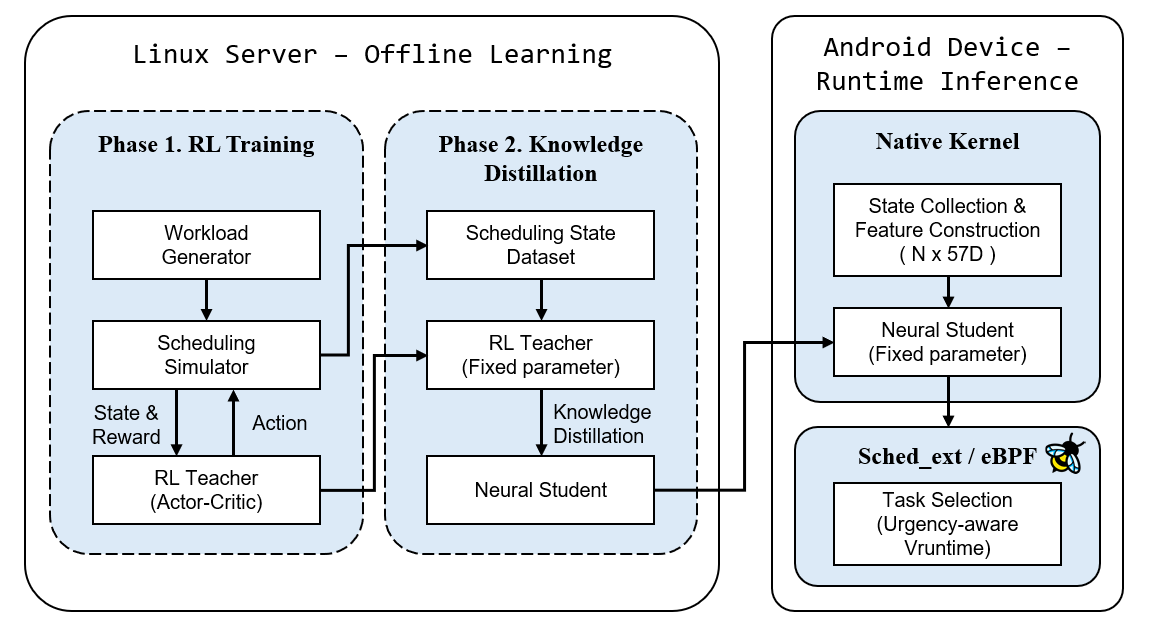
\includegraphics[width=\linewidth,keepaspectratio]{Figures/System_overview.png}%
    }{%
        \fbox{\parbox[c][0.50\linewidth][c]{0.94\linewidth}{%
            \centering System Overview Figure\\
            Upload \texttt{Figures/System\_overview.png} to display the figure.}}%
    }
    \caption{Overall architecture of RL-SchedExt.
    Offline learning consists of RL Teacher training and
    teacher--student knowledge distillation on a Linux server.
    The trained Neural Student is deployed to the Android kernel,
    where its inference results are used for eBPF-based task selection.}
    \label{fig:system_overview}
\end{figure}

\paragraph{Offline Learning.}
Figure~\ref{fig:system_overview}의 Linux Server에서는 Offline Learning을 두 단계로 수행한다.
Phase 1 (RL Teacher Training)에서는 Workload Generator에서 생성한 Workload를 기반으로 Scheduling Simulator를 구성하고, Simulator와의 상호작용을 통해 RL Teacher의 Scheduling Policy를 학습한다.
Simulator는 Kernel에서 관측 가능한 State와 Scheduling Decision에 따른 Deadline-oriented Reward를 제공한다.
Phase 2 (Knowledge Distillation)에서는 Scheduling State Dataset을 학습이 완료된 RL Teacher와 Neural Student에 입력하고, Teacher--Student Knowledge Distillation을 통해 경량 Neural Student를 학습시킨다.
학습된 Neural Student는 INT8 Quantization을 거쳐 Android Kernel에 배포된다.

\paragraph{Runtime Inference.}
Figure~\ref{fig:system_overview}의 Android Device에서는 학습된 Neural Student를 이용하여 Runtime Inference를 수행한다.
Native Kernel은 Runtime State Collection을 통해 Scheduling Event마다 Runtime History를 갱신하고, Task Selection 시점에 Runnable Task Set의 각 Task에 대해 57차원의 State를 구성한다.
Native Kernel의 Neural Student가 Runnable Task Set 내 각 Task의 Learned Vruntime Adjustment를 계산하면, sched\_ext의 eBPF Scheduling Program은 Urgency-aware Vruntime을 기준으로 다음 Task를 선택한다.
Native Kernel은 선택 결과를 검증하여 실제 Task Dispatch에 반영한다. 이러한 구체적인 Runtime 구현 방법은 다음 Chapter에서 설명한다.

RL-SchedExt의 학습 대상은 하나의 CPU에서 경쟁하는 Runnable Task Set의 실행 순서이며, Time Slice와 Preemption은 CFS 방식의 Scheduling Mechanism을 기반으로 처리한다.
Runtime에서는 RL Teacher, Scheduling Simulator 및 Reward 계산이 필요하지 않으며, 학습된 Neural Student의 Weight와 Bias를 고정하여 사용한다.

\section{Simulation-based Learning Environment}
%- Linux Server에서 수행되는 것 설명
%- Simulator 기반 학습 선택한 이유 및 장점
%- 실제 CPU에서의 task execusion과 simulation에서의 차이

실제 Android Kernel에서는 Application Request의 Deadline과 Scheduling Decision의 결과를 학습에 필요한 Reward로 확보하기 어렵다.
또한 실제 Device에서 다양한 Scheduling Policy를 반복적으로 평가하는 데에는 실행 환경의 변동성과 실험 비용이라는 제약이 존재한다.
따라서 RL-SchedExt는 Linux Server에서 가상 시간 기반의 Scheduling Simulator를 이용하여 다양한 Workload와 Scheduling Decision에 따른 실행 결과를 생성한다.
이를 통해 Kernel에서 관측 가능한 State와 Deadline-oriented Reward 사이의 관계를 학습할 수 있는 환경을 구성한다.

\subsection{Workload Modeling}
%- Task 종류 설명 (CPU-bound, Periodic,...) 및 왜 해당 task 종류로 classification했는지
%- Randomized Workload Generation 및 json file output.
실제 시스템에서는 서로 다른 실행 특성과 의존 관계를 가진
Task들이 제한된 CPU 자원을 공유한다.
각 Task는 서로 다른 CPU 실행 특성과 Wakeup Pattern을 가지며,
일부 Task는 다른 Task의 실행 결과나 공유 자원의 상태에 따라
실행 가능 여부가 결정된다.

RL-SchedExt는 이러한 Scheduling 상황을 모사하기 위해
다음과 같은 Task의 실행 특성 및 의존 관계를 모델링한다.

\begin{itemize}
    \item \textbf{CPU-bound:}
    상대적으로 긴 CPU Demand를 가지며 지속적으로
    CPU 자원을 요구하는 실행 특성.

    \item \textbf{I/O-bound:}
    CPU Execution과 I/O Blocking을 반복하며
    빈번한 Sleep 및 Wakeup이 발생하는 실행 특성.

    \item \textbf{Periodic Wakeup:}
    일정한 시간 간격으로 새로운 작업이 Release되는
    실행 특성.

    \item \textbf{Random Burst:}
    불규칙한 시점에 다양한 크기의 CPU Demand가
    발생하는 실행 특성.

    \item \textbf{Chain Dependency:}
    선행 Task의 실행 완료에 따라 후속 Task가 실행 가능한
    상태로 전환되는 순차적 의존 관계.

    \item \textbf{Lock Dependency:}
    공유 자원을 보유한 Task의 Lock Release에 따라
    다른 Task의 실행 가능 여부가 결정되는 의존 관계.
\end{itemize}

Scheduling Simulator는 Task와 Request를 구분하여 관리한다.
Task는 Scheduling Weight, Vruntime, Wakeup Pattern 및 실행 상태를 가지며,
Request는 Arrival Time과 Deadline Budget을 가진다.
Request를 처리하기 위한 CPU Demand는 하나 이상의 Task에 할당되는
실행 작업으로 표현되며, 실행 특성에 따라 Blocking 조건과
Task 간 Dependency가 추가적으로 정의된다.
Absolute Deadline은 Request의 Arrival Time과 Deadline Budget으로부터 결정된다.
Simulator는 이러한 실행 특성과 의존 관계를 조합하여 하나의 Workload를 구성한다.
학습 과정에서는 Task의 수, CPU Demand, Request Arrival Pattern,
Deadline Budget 및 Dependency 등을 Randomization하여
다양한 CPU 경쟁 상황을 생성한다.
이러한 Workload Modeling을 통해 RL Policy가 특정
Application의 실행 패턴에 overfitting되지 않고,
다양한 Task 특성과 의존 관계에서 발생하는 Scheduling
Dynamics를 학습하도록 한다.

\subsection{Modeling CFS Scheduling Dynamics}

Scheduling Simulator는 Linux CFS의 주요 Scheduling
Dynamics를 기반으로 가상의 CPU와 Task의 실행 상태를
관리한다.
실제 Process 또는 Thread를 CPU에서 실행하는 대신,
각 Task를 Scheduling Entity로 표현하고 Simulation Clock을
진행시키면서 Scheduling State를 갱신한다.

각 Scheduling Entity는 현재 처리 중인 실행 작업의 Remaining CPU Demand,
Remaining Time Slice, Vruntime, Scheduling Weight
및 Task State 등의 정보를 유지한다.

Task $i$의 Remaining CPU Demand를 $D_i(t)$,
Remaining Time Slice를 $S_i(t)$,
Vruntime을 $V_i(t)$라고 정의한다.
Task $i$가 $\delta t$만큼 CPU 시간을 할당받으면,
Simulator는 해당 Task가 동일한 양의 CPU 시간을
사용한 것으로 간주한다.

이에 따라 Remaining CPU Demand와 Remaining Time Slice는
다음과 같이 갱신된다.

\begin{equation}
    D_i(t+\delta t)
    =
    \max(0,D_i(t)-\delta t)
\end{equation}
\begin{equation}
    S_i(t+\delta t)
    =
    \max(0,S_i(t)-\delta t)
\end{equation}

Vruntime은 Background에서 설명한 CFS의
Scheduling Weight 기반 CPU Accounting 원리를 적용하여
다음과 같이 갱신된다.

\begin{equation}
    V_i(t+\delta t) = V_i(t)+\delta t\frac{w_0}{w_i}
\end{equation}

여기서 $w_i$는 Task $i$의 Scheduling Weight이며, $w_0$는 Nice-0 Scheduling Weight이다.

Simulation Clock이 진행됨에 따라 Simulator는
Task Release, Wakeup, Blocking, Task Completion 및
Time Slice Expiration 등의 Scheduling Event를 처리한다.
Remaining CPU Demand($D_i(t)$)가 0에 도달하면 해당 실행 작업이
완료된 것으로 처리하며, Request Completion은 해당 Request에
필요한 실행 작업들이 완료되었는지를 기준으로 판단한다.
Remaining Time Slice($S_i(t)$)가 소진되거나
Preemption 조건이 충족되면 새로운 Scheduling Decision을
수행할 수 있다.

I/O Blocking이나 Lock Dependency가 발생한 Task는
Runnable Task Set에서 제외되며,
I/O Completion, Lock Release 또는 선행 Task의 완료 등
실행 가능 조건이 충족되면 Runnable 상태로 전환된다.

CFS를 모사하는 기본적인 Task Selection은
Runnable Task Set $\mathcal{R}(t)$에 대해 다음과 같이
표현할 수 있다.

\begin{equation}
    i^*_{\mathrm{CFS}}
    =
    \arg\min_{i \in \mathcal{R}(t)} V_i(t)
\end{equation}

이러한 Scheduling Dynamics를 기반으로 Simulator는
Task의 실행 순서에 따른 CPU 자원 경쟁, Task 간 의존 관계
및 Completion Time의 변화를 수치적으로 모사한다.

\subsection{Simulation Scope and Abstraction}

Scheduling Simulator는 실제 CPU의 Cache, Memory Stall,
Instruction Execution 등의 Microarchitectural Behavior를
직접적으로 모사하지 않으므로 실제 Device와의
Simulation-to-Reality Gap이 존재할 수 있다.
그러나 RL-SchedExt의 학습 목적은 Hardware 수준의
실행 특성을 정확하게 재현하는 것이 아니라,
Scheduling Decision이 Workload의 실행 결과에 미치는
영향을 학습하는 것이다.
따라서 Simulator는 Hardware-specific Behavior를 추상화하고,
Task의 실행 상태, CPU 자원 경쟁 및 Task 간 의존 관계를
중심으로 Scheduling Environment를 구성한다.
이를 통해 RL Teacher가 다양한 Scheduling Context에서
Task의 실행 순서에 따른 Deadline Miss Count 및 Request Completion Latency의
변화 경향을 학습할 수 있도록 설계하였다.

\section{Reinforcement Learning Formulation}
% - CPU Scheduling의 순차적 의사결정 문제 정의
% - Deadline을 직접 관측할 수 없는 문제
CPU Scheduling은 현재 실행할 Task의 선택이 이후의
Task State와 CPU 경쟁 상황에 영향을 미치는
순차적 의사결정 문제이다.
특히 Task 간 의존 관계가 존재하는 경우,
특정 Task의 실행 순서는 해당 Task가 처리하는 Request의
Completion Time뿐만 아니라 의존 관계에 있는 다른 Task의 실행 가능 시점과
관련 Request의 Deadline 충족 여부에도 영향을 미친다.

그러나 실제 Kernel에서는 Application Request의 Deadline과
미래 CPU Demand를 직접 관측하기 어렵다.
따라서 RL-SchedExt는 Scheduling Simulator에서 제공하는
Deadline 기반 Reward를 이용하여,
Kernel에서 관측 가능한 Runtime State와
Scheduling Decision 사이의 관계를 학습한다.
이를 위해 CPU Scheduling 문제를 State, Action 및
Reward로 구성된 Reinforcement Learning 문제로 정의한다.

\subsection{State: Context-aware Representation}
% - Kernel에서 관측 가능한 Runtime Feature
% - 13D Task Feature 및 6D Global Feature
% - 38D Derived Context Feature
% - 57D State 구성 및 선정 이유
% - Table: State Feature Definition (자세히 설명하는거는 19D만하고 38D 는 derived했다고 표현.
RL-SchedExt는 실제 Kernel에서 수집할 수 있는 Runtime Feature를 기반으로 Task의 실행 특성과 현재 Scheduling Context를 표현한다.
Application Request의 실제 Deadline, Remaining CPU Demand 및 미래 Wakeup 정보는 Runtime State에 포함하지 않는다.

State의 Base Feature는 개별 Task의 실행 특성을 나타내는 13개의
Task Feature와 현재 CPU의 Scheduling 환경을 나타내는 6개의 Global Feature로 구성된다.
Table~\ref{tab:state_features}는 각 Feature의 정의를 보여준다.
여기서 Exponentially Weighted Moving Average (EWMA)는 실행 이력의
이동 평균을, Coefficient of Variation (CV)은 Wakeup Interval의 변동성을
나타낸다.

\begin{table}[t]
    \centering
    \scriptsize
    \setlength{\tabcolsep}{3pt}
    \renewcommand{\arraystretch}{1.15}
    \begin{tabularx}{\linewidth}{|>{\centering\arraybackslash}p{0.08\linewidth}|>{\raggedright\arraybackslash}p{0.32\linewidth}|>{\raggedright\arraybackslash}X|}
        \hline
        \textbf{Dim.} & \textbf{Feature} & \textbf{Description} \\ \hline
        \multicolumn{3}{|c|}{\textbf{Task Features (13D)}} \\ \hline
        1 & Vruntime
          & Virtual Runtime expressed relative to a common reference \\ \hline
        1 & Log2 Weight
          & Log-scaled relative scheduling weight \\ \hline
        1 & CPU Utilization
          & EWMA of CPU execution ratio \\ \hline
        1 & Runnable Ratio
          & EWMA of runnable time ratio \\ \hline
        1 & Current Wait
          & Current runnable waiting time \\ \hline
        1 & Wait EWMA
          & Historical average waiting time \\ \hline
        1 & Wakeup Rate
          & Wakeup frequency \\ \hline
        1 & Time Since Last Run
          & Elapsed time since last execution \\ \hline
        1 & Preemption Rate
          & Preemption frequency \\ \hline
        1 & Sleep/Block Rate
          & Sleep or blocking frequency \\ \hline
        1 & Time Since Quiescent
          & Time since last inactive State \\ \hline
        1 & Wakeup CV
          & Variability of wakeup intervals \\ \hline
        1 & Service Debt
          & CPU service deficit relative to fair share \\ \hline
        \multicolumn{3}{|c|}{\textbf{Global Features (6D)}} \\ \hline
        1 & Runnable Count
          & Number of runnable tasks \\ \hline
        1 & Mean Wait
          & Mean runnable waiting time \\ \hline
        1 & Max Wait
          & Maximum runnable waiting time \\ \hline
        1 & Vruntime Spread
          & Range of runnable Task vruntimes \\ \hline
        1 & CPU Utilization
          & EWMA of CPU utilization \\ \hline
        1 & Context Switch Rate
          & Context switch frequency \\ \hline
        \multicolumn{3}{|c|}{\textbf{Derived Context Features (38D)}} \\ \hline
        5 & Relative Rank
          & Relative feature ranks among runnable tasks \\ \hline
        5 & Relative Difference
          & Feature gaps relative to other tasks
            and aggregate values \\ \hline
        6 & Runnable Task Set Statistics
          & Aggregate statistics of runnable tasks \\ \hline
        6 & Other Task Statistics
          & Statistics excluding the current Task \\ \hline
        5 & First CFS Task
          & Features of the minimum-Vruntime Task \\ \hline
        5 & First CFS Task Difference
          & Feature differences from the first CFS Task \\ \hline
        3 & Second CFS Task
          & Features of the second minimum-Vruntime Task \\ \hline
        3 & Second CFS Task Difference
          & Feature differences from the second CFS Task \\ \hline
        \textbf{57} & \multicolumn{2}{|c|}{\textbf{Total}} \\ \hline
    \end{tabularx}
    \caption{State representation of RL-SchedExt.}
    \label{tab:state_features}
\end{table}

Task Feature는 Task의 CPU 사용 이력, Wakeup Pattern, Runnable Waiting Time 및 CPU 자원 할당 상태를 표현한다.
이를 통해 직접 관측할 수 없는 Task의 실행 특성을
과거 및 현재의 Runtime Behavior로부터 간접적으로
파악할 수 있도록 한다.

Global Feature는 현재 Runnable Task의 수,
대기 시간 및 CPU Utilization 등을 포함하여,
개별 Task의 실행 특성만으로는 표현하기 어려운
CPU 자원 경쟁 상황을 나타낸다.

그러나 동일한 Task Feature를 가지더라도
현재 경쟁하는 다른 Task의 실행 특성에 따라
해당 Task의 Scheduling Urgency는 달라질 수 있다.
예를 들어 동일한 Wakeup Rate를 가진 Task라도
경쟁 Task 대부분이 CPU-bound인 경우와
빈번하게 Wakeup하는 Task인 경우에는
해당 Task를 우선적으로 실행하는 것이 전체 Workload에
미치는 영향이 다를 수 있다.

이러한 상대적인 Scheduling Context를 표현하기 위해
RL-SchedExt는 Base Feature로부터 38개의
Derived Context Feature를 추가적으로 구성한다.
Table~\ref{tab:state_features}에서 나타낸 것과 같이,
Derived Context Feature는 Runnable Task Set의
통계적 특성, 현재 Task의 상대적인 Feature 순위 및
CFS의 Vruntime 기준 첫 번째와 두 번째 실행 우선순위를
가지는 Task와의 비교 정보를 포함한다.
이를 통해 개별 Task의 실행 특성뿐만 아니라
기존 CFS의 Task Ordering와 현재 Task 간의
상대적인 관계를 Policy의 입력으로 제공한다.

최종적으로 Task $i$의 State는 다음과 같이 정의된다.

\begin{equation}
    \mathbf{s}_i = \left[\underbrace{\mathbf{x}_i}_{\text{13D Task}},\ \underbrace{\mathbf{g}}_{\text{6D Global}},\ \underbrace{g_{\mathrm{ctx}}(\mathbf{x}_i,\mathbf{g},\mathcal{R}_k)}_{\text{38D Derived}}\right] \in \mathbb{R}^{57}
    \label{eq:state_representation}
\end{equation}

여기서 $\mathcal{R}_k=\mathcal{R}(t_k)$는 실제 시각 $t_k$에서
Scheduling Decision Step $k$에 사용되는 Runnable Task Set이며,
$g_{\mathrm{ctx}}$는 Context Feature Extraction Function이다.
Scheduling State $S_k$는 해당 Runnable Task Set에 포함된 각 Task의
57차원 State를 Task Index에 대응시킨 집합 표현이다.

\begin{equation}
    S_k = (\mathbf{s}_i)_{i\in\mathcal{R}_k}
    \label{eq:scheduling_state}
\end{equation}

이후 실제 시각은 $t$, Scheduling Decision Step은 $k$로 구분한다.
실제 구현에서 Runnable Task Set이 지원 범위를 초과할 경우에는
Chapter~4에서 설명하는 Fallback Selection Path를 사용한다.

따라서 Neural Student의 57차원 State는 57개의 독립적인
Kernel 정보를 수집하는 것이 아니라,
19개의 Base Feature와 이들로부터 계산된 38개의
Derived Context Feature로 구성된다.
이러한 State Representation은 개별 Task의 실행 특성과
Task 간 상대적인 관계를 함께 표현함으로써,
현재 Scheduling Context에 따른 Learned Vruntime Adjustment를
학습할 수 있도록 설계되었다.


\subsection{Action: Urgency-aware Task Ordering}
% - RL Action 정의
% - Learned Vruntime Adjustment
% - Urgency-aware Vruntime 계산 공식 : Vruntime + Learned Vruntime Adjustment
% - Task Selection 공식 : min(Urgency-aware Vruntime) 

RL-SchedExt의 Action은 현재 Runnable Task Set에서
다음 실행할 Task를 선택하는 것으로 정의된다.
이를 위해 Policy는 각 Task의 State와 Scheduling Context를
기반으로 Learned Vruntime Adjustment($\Delta V_i$)를 계산한다.

\begin{equation}
    \Delta V_i = f_{\theta}(\mathbf{s}_i,\mathcal{R}_k)
    \label{eq:learned_adjustment}
\end{equation}

여기서 $f_{\theta}$는 학습된 Scheduling Policy, $\mathbf{s}_i$는 Task $i$의 State,
$\mathcal{R}_k$는 Scheduling Decision Step $k$의 Runnable Task Set이다.

기존 Vruntime에 Learned Vruntime Adjustment를
반영한 값을 Urgency-aware Vruntime으로 정의한다.

\begin{equation}
    \underbrace{V_i^{\mathrm{urgency}}}
        _{\text{Urgency-aware Vruntime}}
    =
    \underbrace{V_i}
        _{\text{Vruntime}}
    +
    \underbrace{\Delta V_i}
        _{\text{Learned Vruntime Adjustment}}
    \label{eq:urgency_aware_vruntime}
\end{equation}

Learned Vruntime Adjustment는 Task의 Scheduling Urgency를
기존 Fairness 기반 Task Ordering에 반영하기 위한 조정값이다.
다른 조건이 동일할 때 음의 Adjustment는 Task의 Scheduling Priority를
높이며, 양의 Adjustment는 Scheduling Priority를 낮춘다.

Runtime Inference에서는 Runnable Task Set $\mathcal{R}_k$ 내에서
가장 작은 Urgency-aware Vruntime을 가지는 Task를
다음 실행 대상으로 선택한다.

\begin{equation}
    a_k =
    \underset{i\in\mathcal{R}_k}{\arg\min}
    V_i^{\mathrm{urgency}}
    \label{eq:task_selection}
\end{equation}

Learned Vruntime Adjustment는 기존 Vruntime의
Accounting 값을 변경하지 않으며,
Task Selection에만 사용된다.
본 논문에서는 Scheduling 원리의 설명을 위해 개념적인 Vruntime $V_i$를
사용한다. 실제 구현에서는 Runnable Task Set 전체에 공통된 기준 Vruntime을
차감한 값을 사용하지만, 동일한 기준값을 차감하므로 Task Ordering은
변하지 않는다.


\begin{table}[t]
    \centering
    \small
    \setlength{\tabcolsep}{3pt}
    \renewcommand{\arraystretch}{1.15}
    \begin{tabularx}{\linewidth}{|>{\centering\arraybackslash}p{0.18\linewidth}|>{\centering\arraybackslash}X|>{\centering\arraybackslash}p{0.16\linewidth}|}
        \hline
        \textbf{Symbol} & \textbf{Reward Component} & \textbf{Reward Weight} \\ \hline
        \multicolumn{3}{|c|}{
            \textbf{Primary Reward Components}} \\ \hline
        $R_k^{\mathrm{req}}$
            & Completed Request Reward & $+1.0$ \\ \hline
        $M_j$
            & Deadline Miss & $-3.0$ \\ \hline
        $O_j$
            & Deadline Overrun & $-1.5$ \\ \hline
        $L_j$
            & Request Completion Latency & $-0.3$ \\ \hline
        \multicolumn{3}{|c|}{
            \textbf{Auxiliary Reward Components}} \\ \hline
        $B_k$
            & Background CPU Service (ms) & $+0.12$ \\ \hline
        $W_k$
            & Runnable Waiting Time (ms) & $-0.015$ \\ \hline
        $U_k$
            & Wakeup-to-run Latency (ms) & $-0.04$ \\ \hline
        $H_k$
            & Context Switch Overhead (ms) & $-0.12$ \\ \hline
        $N_k^{\mathrm{switch}}$
            & Context Switch Count & $-0.003$ \\ \hline
        $R_k^{\mathrm{end}}$
            & Unfinished Work Penalty & $+1.0$ \\ \hline
    \end{tabularx}
    \caption{Reward components and their weights.}
    \label{tab:reward_components}
\end{table}

\subsection{Reward: Deadline-oriented Optimization}
% - Reward function 전체 공식 설명
% - Deadline Miss, Deadline Overrun, Request Completion Latency 구성요소 설명 하면서 Deadline miss만 최적화 하면 안되는 이유 간단 설명.
% - Reward Component별 Weight 및 Normalization

RL-SchedExt는 Deadline Miss, Deadline Overrun 및
Request Completion Latency를 주요 Optimization Objective로 설정한다.
또한 Background CPU Service, Runnable Waiting Time,
Wakeup-to-run Latency 및 Scheduling Overhead를 고려하여
Step Reward를 다음과 같이 정의한다.

\begin{equation}
    r_k = R_k^{\mathrm{req}} + \lambda_b B_k - \lambda_w W_k - \lambda_u U_k - \lambda_o H_k - \lambda_s N_k^{\mathrm{switch}} + R_k^{\mathrm{end}}
    \label{eq:total_reward}
\end{equation}

Table~\ref{tab:reward_components}는 전체 Reward Function의
각 Component와 적용되는 Reward Weight를 나타낸다.

Request Reward는 Application Request가 완료되는 시점에
해당 Request의 실행 결과를 기반으로 계산된다.
Background에서 정의한 성능 지표를 이용하여
Request $j$에 대한 Reward를 다음과 같이 정의한다.

\begin{equation}
    R_j =
    -\underbrace{\alpha M_j}_{\text{Deadline Miss}}
    -\underbrace{\beta O_j}_{\text{Deadline Overrun}}
    -\underbrace{\gamma L_j}_{\text{Request Completion Latency}}
    \label{eq:request_reward}
\end{equation}

Scheduling Decision Step $k$부터 다음 Step까지
완료된 Request의 집합을 $\mathcal{J}_k$라고 하면,
해당 구간의 Request Reward는 다음과 같이 계산된다.

\begin{equation}
    R_k^{\mathrm{req}}
    =
    \sum_{j\in\mathcal{J}_k}R_j
    \label{eq:request_reward_sum}
\end{equation}

% \clearpage
\section{Neural Policy Learning and Distillation}
% - Scheduling Performance와 Inference Cost의 Trade-off
% - Teacher-Student 구조의 설계 목적
% - Figure RL Teacher 와 Student network 구조그리기
Figure~\ref{fig:teacher_student_architecture}는 RL Teacher Training과 Knowledge Distillation으로 구성된 두 단계의 Offline Learning 과정을 나타낸다.

\begin{figure}[H]
    \centering

    \begin{subfigure}[b]{0.49\linewidth}
        \centering
        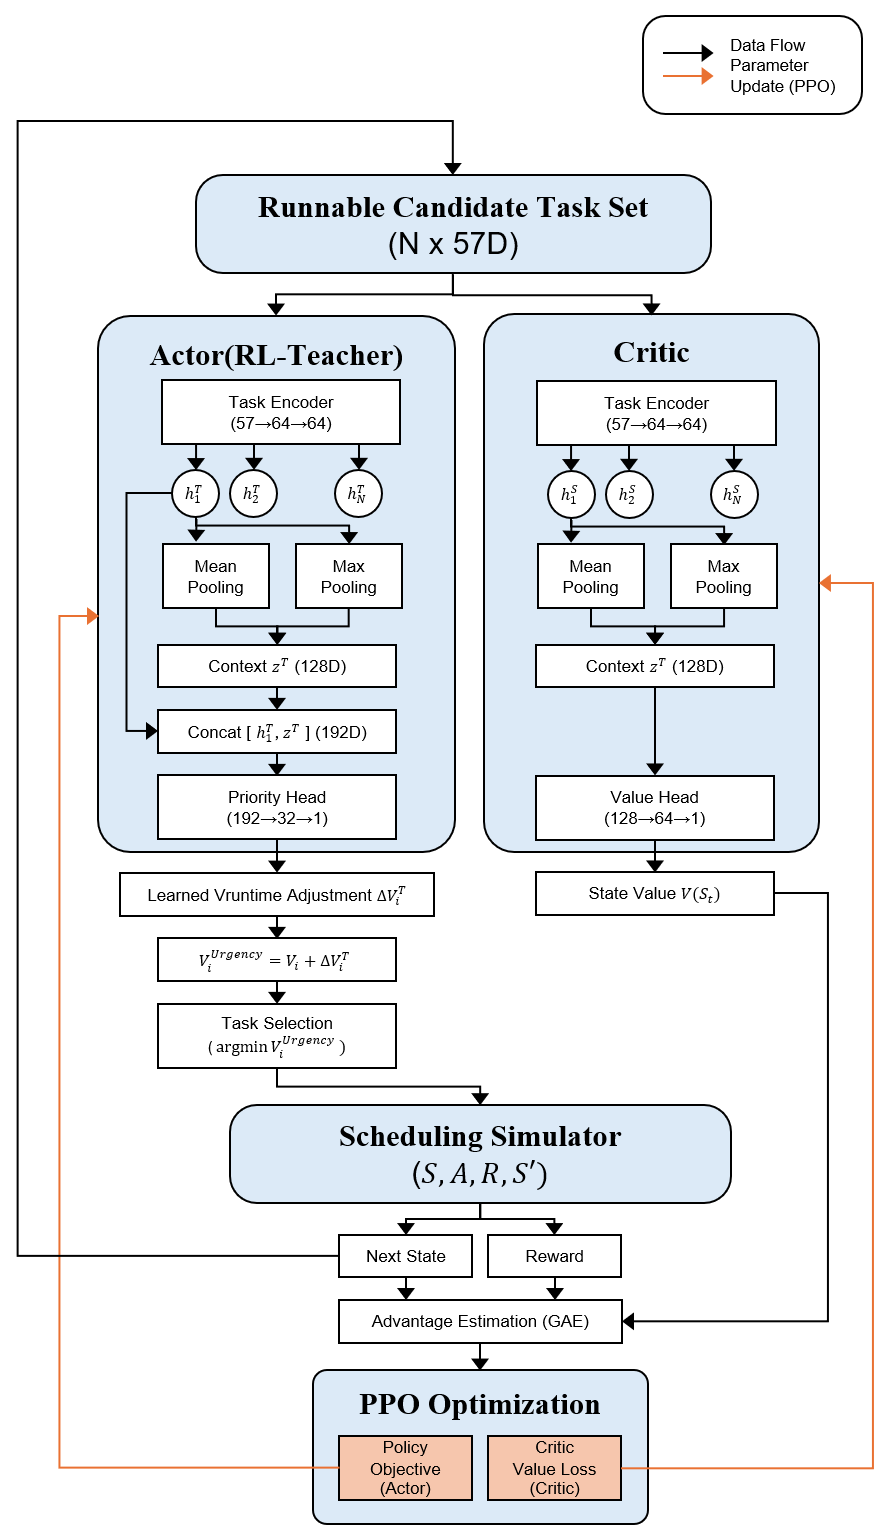
\includegraphics[
            width=\linewidth,
            keepaspectratio
        ]{Figures/ActorCritic.png}
        \caption{Phase 1: RL Teacher Training}
        \label{fig:actor_critic}
    \end{subfigure}
    % \hfill
    \hspace{1pt}%
    \begin{subfigure}[b]{0.49\linewidth}
        \centering
        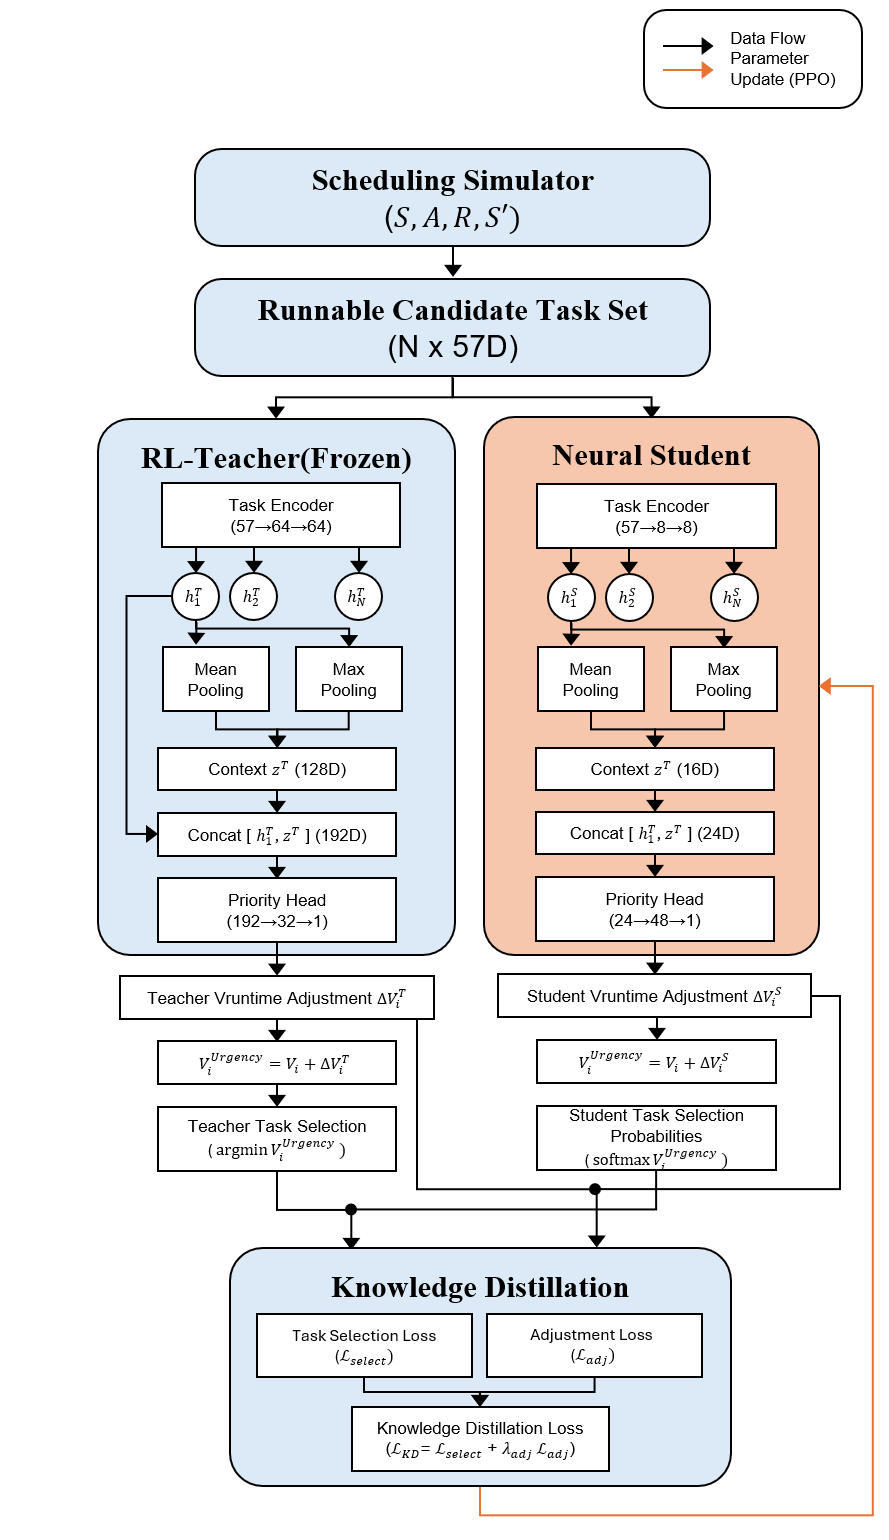
\includegraphics[
            width=\linewidth,
            keepaspectratio
        ]{Figures/TeacherStudent.png}
        \caption{Phase 2: Knowledge Distillation}
        \label{fig:teacher_student}
    \end{subfigure}

    \caption{RL-SchedExt의 2단계 Offline Learning Framework.
    Phase 1 (RL Teacher Training)에서는 RL Teacher가 Scheduling Simulator와의
    상호작용을 통해 문맥 의존적(Context-dependent)
    Scheduling Policy를 학습한다.
    Phase 2 (Knowledge Distillation)에서는 RL Teacher의 Weight와 Bias를 고정한 상태에서
    지식 증류(Knowledge Distillation)를 통해 학습된 Policy를
    경량 Neural Student에 전달한다.}
    \label{fig:teacher_student_architecture}
\end{figure}

\subsection{RL Teacher Policy}
% - Teacher Neural Network Architecture
% - Actor-Critic Architecture
% - Context Encoding 및 Policy Output
% - PPO 기반 Policy Optimization
RL Teacher Training에서는 다양한 Scheduling Context에서
Deadline-oriented Scheduling Policy를 학습하기 위해
DeepSets 기반의 Actor--Critic Architecture를 사용한다.
Figure~\ref{fig:teacher_student_architecture}(\subref{fig:actor_critic})는 RL Teacher의
Network Architecture와 Proximal Policy Optimization (PPO) 기반의 학습 과정을 나타낸다.

\paragraph{Actor Network Architecture.}
Actor는 현재 Runnable Task Set을 입력받아
각 Task의 Learned Vruntime Adjustment를 계산한다.
각 Task의 57차원 State는 공유된 Task Encoder를 통해
64차원의 Task Embedding으로 변환된다.

\begin{equation}
    \mathbf{h}_i^T = \phi_T(\mathbf{s}_i) \in \mathbb{R}^{64}
\end{equation}

여기서 $\phi_T$는 $57 \rightarrow 64 \rightarrow 64$ 구조의 Task Encoder이다.

각 Task Embedding에 대해 Mean Pooling과 Max Pooling을
수행하여 전체 Runnable Task Set의
특성을 나타내는 128차원의 Set Context를 구성한다.

\begin{equation}
    \mathbf{z}^T = \left[\underset{i\in\mathcal{R}_k}{\operatorname{Mean}}(\mathbf{h}_i^T),\ \underset{i\in\mathcal{R}_k}{\operatorname{Max}}(\mathbf{h}_i^T)\right] \in \mathbb{R}^{128}
\end{equation}

 개별 Task의 Embedding과 전체 Set Context를 결합한
192차원의 Vector는 Adjustment Head의 입력으로 사용된다.
Adjustment Head는 개별 Task의 실행 특성과
전체 Scheduling Context를 기반으로
 Learned Vruntime Adjustment를 계산한다.

\begin{equation}
    \Delta V_i^T = B\tanh\left(\psi_T([\mathbf{h}_i^T,\mathbf{z}^T])\right)
\end{equation}

여기서 $\psi_T$는 $192 \rightarrow 32 \rightarrow 1$ 구조의 Adjustment Head이며, $B$는 Adjustment Bound이다.

\paragraph{Stochastic Task Selection.}
학습 과정에서는 Urgency-aware Vruntime을 기반으로
각 Task의 선택 확률을 계산한다.

\begin{equation}
    \pi_{\theta}(i\mid S_k)
    =
    \frac{
        \exp(-V_i^{\mathrm{urgency}}/\tau_T)
    }{
        \sum_{j\in\mathcal{R}_k}
        \exp(-V_j^{\mathrm{urgency}}/\tau_T)
    }
    \label{eq:teacher_policy}
\end{equation}

여기서 $\tau_T$는 Task Selection 확률 분포를 조절하는 Temperature이다.
RL Teacher Training에서는 해당 확률 분포로부터 실행할 Task를 확률적으로 선택하며,
Scheduling Simulator는 선택된 Task의 실행 결과를
기반으로 Next State와 Reward를 생성한다.

\paragraph{Critic Network.}
Critic은 Actor와 동일한 Scheduling State를 입력받으며,
독립적인 Task Encoder와 Set-context Pooling을 통해
전체 Scheduling Context를 구성한다.
Value Head는 현재 Scheduling State에서 기대되는
누적 Reward인 State Value를 추정한다.

\begin{equation}
    V_{\omega}(S_k) = \mathbb{E}_{\pi}[G_k\mid S_k]
\end{equation}

여기서 $G_k$는 Discounted Cumulative Reward이다.

\paragraph{PPO-based Policy Optimization.}
Critic이 추정한 State Value와 Scheduling Simulator에서
수집된 Reward를 기반으로 Generalized Advantage
Estimation (GAE)을 수행한다.
이를 통해 Actor의 Scheduling Decision이
기존 Policy의 기대 결과인 State Value보다 얼마나 좋은지를 나타내는
Advantage를 예측한다.

RL Teacher는 PPO를
이용하여 Actor와 Critic의 Weight와 Bias를
최적화한다.
Actor의 Clipped Policy Objective는 다음과 같으며 
Actor의 Policy를 어떤 방향으로, 얼마나 개선할 것인지 결정한다.

\begin{equation}
    J_{\mathrm{PPO}}(\theta) = \mathbb{E}_k\left[\min\left(\eta_k(\theta)\widehat{A}_k,\ \operatorname{clip}(\eta_k(\theta),1-\epsilon,1+\epsilon)\widehat{A}_k\right)\right]
\end{equation}

\begin{equation}
    \eta_k(\theta) = \frac{\pi_{\theta}(a_k\mid S_k)}{\pi_{\theta_{\mathrm{old}}}(a_k\mid S_k)}
\end{equation}

여기서 $\eta_k(\theta)$는 새로운 Scheduling Policy와 이전 Scheduling Policy의
Task Selection 확률 비율이며, $\widehat{A}_k$는 Estimated Advantage,
$\epsilon$은 PPO Clipping Parameter이다.

Actor는 높은 Advantage를 가지는 Scheduling Decision의
선택 확률을 증가시키는 방향으로 학습되며,
Clipping을 통해 Policy의 급격한 변화를 억제한다.
Critic은 Scheduling Simulator에서 수집된 Reward와
각 State에서 추정한 State Value를 기반으로
Value Target을 계산하고, 추정한 State Value와
Value Target 간의 오차를 최소화하도록 학습된다.

이러한 Simulator-based RL Training을 반복하여 RL Teacher는
기대 누적 Reward를 최대화하는 Scheduling Policy를
학습한다.

\subsection{Lightweight Neural Student}
% - Neural Student Architecture
% - Task Encoder, Set-context Pooling, Adjustment Head
% - Nonlinear Feature Interaction
% - Deepsets : Candidate Task 수 및 순서에 대한 유연성
% - Per-task Learned Vruntime Adjustment
Neural Student는 RL Teacher가 학습한 Nonlinear
Scheduling Policy를 Kernel의 제한된 연산 환경에서
실행하기 위한 경량 Neural Network이다.
RL Teacher의 Actor와 동일한 DeepSets Architecture를
유지하면서 Task Encoder와 Adjustment Head의
Network Dimension을 재구성하여 Inference에
필요한 연산량을 감소시킨다.

Task Encoder의 구조를
$57 \rightarrow 64 \rightarrow 64$에서
$57 \rightarrow 8 \rightarrow 8$로 축소하여
Task Embedding의 Dimension을 64에서 8로 감소시킨다.
이에 따라 Mean/Max Pooling을 통해 구성되는
Set Context는 128차원에서 16차원으로 감소하며,
Adjustment Head의 입력은 192차원에서 24차원으로 감소한다.
Adjustment Head는 $24 \rightarrow 48 \rightarrow 1$의
구조로 구성된다.

Neural Student는 Network의 경량화에도 불구하고
Nonlinear Activation과 Set-context Pooling을 유지하여
State Feature 간의 Nonlinear Interaction과
Runnable Task Set 내 Task 간의 상대적인 Scheduling Context를
반영할 수 있다.
Neural Student의 Weight 수는 1,720개로,
RL Teacher의 Actor 대비 Fully Connected Layer의
연산량을 약 87.6\% 감소시킨다.
추가적으로 INT8 Quantization을 적용하여
Kernel 내부에서 Integer 기반의 Inference를 수행한다.

\subsection{Teacher--Student Knowledge Distillation}
% - Teacher와 Student의 Input/Output 관계
% - Teacher Policy의 Knowledge Transfer
% - Distillation Loss 공식
% - Task 간 상대적인 Priority 관계 학습
Figure~\ref{fig:teacher_student_architecture}(\subref{fig:teacher_student})는
학습된 RL Teacher의 Scheduling Policy를 Neural Student로 전달하는
Knowledge Distillation 과정을 나타낸다.
학습이 완료된 RL Teacher의 Weight와 Bias를
고정한 상태에서 RL Teacher와 Neural Student에 동일한
Scheduling State를 입력한다.
RL Teacher의 Task별 Learned Vruntime Adjustment와
RL Teacher의 Task Selection 결과는 Neural Student의
학습 목표로 사용된다.

RL Teacher와 Neural Student의 Urgency-aware Vruntime은
각각 다음과 같이 정의된다.

\begin{equation}
    V_i^T = V_i + \Delta V_i^T,\qquad V_i^S = V_i + \Delta V_i^S
\end{equation}

Knowledge Distillation에서는 각 모델의 Urgency-aware Vruntime이 가장 작은
Task를 해당 모델의 Task Selection 결과로 정의한다.
RL Teacher의 Task Selection 결과와 Neural Student의 Task Selection 결과는
각각 다음과 같다.

\begin{equation}
    i_T^* =
    \underset{i\in\mathcal{R}_k}{\arg\min}\ V_i^T,\qquad
    i_S^* =
    \underset{i\in\mathcal{R}_k}{\arg\min}\ V_i^S
\end{equation}

Distillation Loss는 Neural Student의 Task Selection 결과가 RL Teacher의
Task Selection 결과와 일치하도록 학습하는 Task Selection Loss와
각 Task의 Learned Vruntime Adjustment를 학습하기 위한
Adjustment Regression Loss로 구성된다.

\paragraph{Task Selection Loss.}
Neural Student의 Urgency-aware Vruntime을 기반으로
각 Task의 선택 확률을 계산한다.

\begin{equation}
    p_i^S =
    \frac{
        \exp(-V_i^S/\tau_S)
    }{
        \sum_{j\in\mathcal{R}_k}\exp(-V_j^S/\tau_S)
    }
\end{equation}

여기서 $\tau_S$는 Neural Student의 Temperature이다.
RL Teacher의 Task Selection 결과를 학습 목표로 하여
Cross-entropy Loss를 다음과 같이 정의한다.

\begin{equation}
    \mathcal{L}_{\mathrm{select}}
    =
    -\log p_{i_T^*}^S
\end{equation}

\paragraph{Adjustment Regression Loss.}
RL Teacher가 계산한 Runnable Task Set 내 각 Task의
Learned Vruntime Adjustment를 재현하기 위해
RL Teacher와 Neural Student의 출력 간 Mean Squared Error
(MSE)를 계산한다.

\begin{equation}
    \mathcal{L}_{\mathrm{adj}}
    =
    \frac{1}{|\mathcal{R}_k|}
    \sum_{i\in\mathcal{R}_k}
    \left(
        \Delta V_i^S-\Delta V_i^T
    \right)^2
\end{equation}

최종 Distillation Loss는 다음과 같이 정의된다.

\begin{equation}
    \mathcal{L}_{\mathrm{KD}}
    =
    \underbrace{\mathcal{L}_{\mathrm{select}}}
        _{\text{Task Selection}}
    +
    \underbrace{\lambda_{\mathrm{adj}}
        \mathcal{L}_{\mathrm{adj}}}
        _{\text{Adjustment Regression}}
    \label{eq:distillation_loss}
\end{equation}

두 Loss를 결합함으로써 Neural Student는 개별 Task의 Learned Vruntime Adjustment와 RL Teacher의 Task Selection 결과를 함께 학습한다. 이는 경량 Network에서도 RL Teacher의 Context-dependent Scheduling Policy를 유지하기 위한 것이다.


\chapter{Implementation}
\section{In-Kernel Neural Policy Inference}
\label{sec:implementation}
\label{sec:in_kernel_inference}

RL-SchedExt는 Android 15의 Linux 6.1 Kernel에
Backport된 sched\_ext Framework를 기반으로 구현하였다.
학습된 Neural Student의 Runtime 실행 과정은
Runtime State Collection, Student Neural Policy Inference 및
eBPF Scheduling Decision으로 구성된다.

RL-SchedExt는 기존 sched\_ext의 Task Lifecycle 및 Dispatch 경로에
Native Kernel 기반의 State Collection과 Neural Network Inference를
통합하고, Task Selection을 위한 eBPF Callback을 추가하였다.
Scheduling Decision에 필요한 Feature Construction 및
Neural Network 연산은 Native Kernel에서 수행하며,
eBPF Program에는 각 Candidate의 Vruntime Lag와
Learned Vruntime Adjustment를 전달한다.
이를 통해 eBPF Verifier의 Program Complexity 및 Stack 제약에
대한 부담을 줄이면서 Scheduling Policy의 최종 Task Selection은
eBPF Program에서 수행할 수 있다.
별도의 User Space Inference Daemon과 Runtime 학습은 필요하지 않다.

본 구현의 Neural Policy는 CPU7의 Local Dispatch Queue (DSQ)를
대상으로 동작한다.
따라서 본 연구의 적용 범위는 하나의 CPU에서 경쟁하는
Runnable Task의 실행 순서를 결정하는 것이며,
CPU Selection 및 Load Balancing을 학습하는 것은 아니다.

% Implementation reference:
% android-gs-caimito-6.1-android15-qpr2-beta
% integration/ctx5-tiny-linear-v6-20261122
% aosp/kernel/sched/ext.c, scx_rl_ctx5_native.h,
% scx_rl_ctx5_native_history.h, scx_rl_ctx5_tiny.h
% aosp/tools/sched_ext/include/scx/rl_ctx5_export_core.h,
% rl_ctx5_tiny_infer.h, rl_ctx5_tiny.bpf.h
% aosp/tools/sched_ext/scx_simple.bpf.c

\subsection{Runtime State Collection}

\paragraph{Event-driven Runtime History.}
System Design에서 정의한 State Feature는 단일 Scheduling Event에서
모두 관측할 수 있는 정보가 아니다.
예를 들어 Wakeup Rate와 CPU Utilization은 일정 기간의 실행 이력이
필요하며, Current Wait는 Task가 Runnable 상태로 전환된 시점과
실제로 실행되는 시점 사이의 시간 정보를 필요로 한다.
따라서 RL-SchedExt는 Native Kernel에서 Task별 Runtime History를
관리하고, Scheduling Event가 발생할 때 관련 정보를 갱신한다.

Table~\ref{tab:runtime_events}는 State Collection을 위해 추가한
Native Kernel Event와 주요 갱신 정보를 나타낸다.
Task History는 PID와 Task의 생성 시각을 함께 사용하여 식별하며,
Task의 Scheduling Class 또는 CPU 소속이 변경되는 경우
기존 History의 유효성을 관리한다.
Native Policy Mode에서는 eBPF의 기존 History 갱신 경로를
사용하지 않아 동일 Event가 중복으로 반영되지 않도록 한다.

\begin{table}[htbp]
    \centering
    \small
    \renewcommand{\arraystretch}{1.15}
    \begin{tabularx}{\linewidth}{|p{0.24\linewidth}|X|}
        \hline
        \textbf{Scheduling Event} & \textbf{Runtime History Update} \\ \hline
        Runnable & Runnable transition, waiting start, wakeup history \\ \hline
        Running & Waiting time, execution start, context switch history \\ \hline
        Stopping & Execution accounting, preemption history, waiting state \\ \hline
        Quiescent & Sleep/block history, runnable state removal \\ \hline
        Weight Change & Scheduling weight and service accounting \\ \hline
        Reset & Task history initialization or invalidation \\ \hline
    \end{tabularx}
    \caption{Runtime history updates on scheduling events.}
    \label{tab:runtime_events}
\end{table}

CPU Utilization과 Runnable Ratio는 시간에 따른
Exponentially Weighted Moving Average (EWMA)를 이용하여 관리한다.
Wakeup 등의 빈도 정보는 제한된 크기의 Timestamp Ring을
이용하여 계산한다.
CPU Execution Time 및 Scheduling Weight를 기반으로
각 Task에 기대되는 CPU Service와 실제 제공된 CPU Service의
차이를 누적하여 Service Debt를 구성한다.
이와 같이 Event-driven Accounting을 사용함으로써
Scheduling Decision마다 과거의 전체 실행 이력을
다시 탐색할 필요가 없다.

\paragraph{Shadow Vruntime Accounting.}
sched\_ext에서 관리하는 Dispatch Queue의 Virtual Time은
CFS Scheduling Entity의 Vruntime과 동일한 Accounting 값이 아니다.
또한 Task가 sched\_ext Scheduling Class에서 실행되는 동안
CFS의 Vruntime이 기존 CFS 실행 경로와 동일하게
갱신된다고 가정할 수 없다.
따라서 RL-SchedExt는 CFS 기반 Scheduling Policy를 학습한
Neural Student의 입력과 Task Selection에 사용하기 위해
별도의 Shadow Vruntime을 관리한다.

Task $i$가 $\Delta t_i$ 동안 실행된 경우
Shadow Vruntime은 다음과 같이 갱신한다.

\begin{equation}
    V_i^{\mathrm{shadow}} \leftarrow
    V_i^{\mathrm{shadow}} +
    \Delta t_i \frac{w_{\mathrm{ref}}}{w_i}.
    \label{eq:shadow_vruntime}
\end{equation}

여기서 $w_i$는 sched\_ext Scheduling Weight이며,
$w_{\mathrm{ref}}$는 기준 Weight이다.
실행 시간에 따른 Weighted Accounting과 Wakeup 시의
Vruntime Placement를 별도로 관리하여
CFS의 주요 Virtual Runtime Dynamics를 모사한다.
Learned Vruntime Adjustment는 이러한 Accounting 과정에
반영하지 않는다.

Scheduling Decision 시점에는 Candidate Task Set의
최소 Shadow Vruntime을 기준으로 Vruntime Lag를 계산한다.

\begin{equation}
    \ell_i = V_i^{\mathrm{shadow}} -
    \min_{j\in\mathcal{C}} V_j^{\mathrm{shadow}}.
    \label{eq:runtime_vruntime_lag}
\end{equation}

이를 통해 절대적인 Vruntime 값 대신 Candidate Task 간의
상대적인 CPU Service 차이를 State Feature로 사용한다.
이 Shadow Accounting은 CFS의 주요 동작을 모사하는 것이며,
CFS의 전체 Scheduling Hierarchy와 동작을
완전히 동일하게 재현하는 것은 아니다.

\paragraph{Candidate Collection and State Construction.}
Task Selection 시점에는 Runqueue Lock을 유지한 상태에서
Local DSQ에 존재하는 Task 중 현재 CPU에서 실행 가능한
Candidate를 수집한다.
Scheduling Class, Runnable 상태 및 CPU Affinity를 확인하고,
Task Identity를 포함하는 Scheduling Context를 구성한다.
History가 유효하지 않거나 Candidate 수가 최대 16개를
초과하는 경우에는 일부 Candidate만을 이용하여
Neural Policy를 실행하지 않는다.

수집된 Candidate의 Runtime History를 현재 시각까지 갱신한 후,
13차원 Task Feature와 6차원 Global Feature를 추출한다.
Task Set의 Feature 합계, 최댓값 및 최소 Vruntime을 가지는
첫 번째와 두 번째 Candidate 등의 공통 정보는
Scheduling Decision마다 한 번만 계산한다.
이 정보를 각 Task의 State Construction에서 재사용하며,
Task별 상대 순위와 다른 Candidate와의 Feature 차이를
계산하여 38차원 Derived Context Feature를 구성한다.

최종 State는 Simulator에서 정의한 Android Feature Representation과
동일한 Feature 순서 및 Scaling을 사용하여
57차원의 Signed Q10 Vector로 변환한다.
State의 Feature Scaling과 Saturation은
Runtime에서 학습 시 사용한 입력 범위를 유지하기 위한 것이다.
이 과정에서 Application-level Deadline이나
Request Completion 정보는 사용하지 않는다.

\subsection{Student Neural Policy Inference}

\paragraph{Integer-only Neural Inference.}
Kernel Scheduling Context에서는 Floating-point 연산의 사용에
제약이 있으므로, 학습된 Neural Student를
Integer 연산 기반의 Network로 변환하였다.
학습 완료 후 Fully Connected Layer의 Weight를
Output Channel별 Symmetric INT8 형식으로 양자화하며,
Scale은 Q24, Bias와 Intermediate Activation은 Q10 형식으로
표현한다.
양자화된 Model Parameter와 Activation 계산에 필요한
정적 배열은 C Header 형태로 Kernel에 포함한다.

각 Fully Connected Layer의 Output Channel $o$는
다음과 같은 Fixed-point 연산으로 계산된다.

\begin{equation}
    y_o^{\mathrm{Q10}} =
    \operatorname{round}
    \left(
        \frac{
            m_o^{\mathrm{Q24}}\sum_j
            x_j^{\mathrm{Q10}}q_{o,j}
        }{2^{24}}
    \right)+b_o^{\mathrm{Q10}},
    \label{eq:student_integer_affine}
\end{equation}

여기서 $q_{o,j}$는 INT8 Weight,
$m_o^{\mathrm{Q24}}$는 Output Channel별 Scale이며,
$b_o^{\mathrm{Q10}}$는 Bias이다.
곱셈 및 누산에는 Signed 64-bit Integer를 사용하고,
Fixed-point 변환에는 Round-half-away-from-zero 규칙을 적용한다.
연산 중 Overflow가 발생한 경우에는 해당 결과를 사용하지 않는다.

Tanh Activation은 입력을 $[-4,4]$ 범위로 제한한 후,
Q10 간격으로 미리 계산된 8,193개의 값을 조회하여 수행한다.
따라서 Scheduling Hot Path에서 Floating-point 연산이나
Exponential Function 계산이 필요하지 않다.
이 Table은 Scheduling Policy가 아니라 Activation Function을
구현하기 위한 것으로, Neural Network의 Weight와
Set-context 연산은 그대로 유지된다.

\paragraph{Bounded Inference and Fast Path.}
DeepSets 구조에서는 각 Task의 Embedding을 계산한 후
전체 Candidate Task Set의 Context를 구성해야 한다.
이에 따라 Native Kernel의 Forward Pass를
Task Encoding, Mean/Max Pooling 및 Priority Head의
세 단계로 분리하였다.
전체 Candidate의 Embedding을 먼저 계산하여 저장하고,
Set Context는 한 번만 계산하여 각 Task의 Priority Head에서
공통으로 사용한다.

최대 Candidate 수를 16개로 제한하고,
Input State와 Intermediate Activation을 저장하기 위한
Scratch Buffer를 사전에 확보한다.
이를 통해 Runqueue Lock을 유지한 Scheduling Hot Path에서
동적 Memory Allocation을 수행하지 않는다.
Fully Connected Layer의 연산량은 Candidate 수 $N$에 대해
$1{,}720N$ MAC으로 증가하며,
Feature Construction의 Task별 상대 순위 계산에는
별도의 Candidate 간 비교가 필요하다.

또한 일반적인 Next-task Selection에서 Candidate가 하나뿐인 경우에는
Priority Adjustment가 Task Selection 결과를 변경할 수 없다.
따라서 단일 Candidate에 대해서는 State Construction 및
유효성 확인 이후 Neural Network의 Forward Pass를 생략하고,
0의 Adjustment를 전달하는 Fast Path를 구현하였다.
이는 Wakeup 평가나 Audit Mode까지 생략하는 방식은 아니다.

Priority Head의 출력은 $\pm 2$\,ms 범위로 제한하며,
Nanosecond 단위의 정수로 변환한다.
계산된 Adjustment와 Candidate별 Valid Flag를
Scheduling Context에 기록한 후 eBPF Program으로 전달한다.

\subsection{eBPF Scheduling Decision}

\paragraph{Task Selection Callback.}
기존 sched\_ext의 Local DSQ 기반 Task Selection 경로에
RL-SchedExt의 Task Selection Callback인
\texttt{rl\_choose}를 추가하였다.
Native Kernel은 다음 Task를 선택해야 하는 시점에
Candidate Collection과 Neural Inference를 수행하고,
\texttt{scx\_rl\_pick\_ctx}를 통해
Candidate의 Vruntime Lag, Learned Adjustment 및
유효성 정보를 eBPF Program에 전달한다.

eBPF Program은 전달된 Candidate에 대해
Equation~\ref{eq:urgency_aware_vruntime}에 대응하는
Scheduling Key를 계산한다.

\begin{equation}
    K_i = \ell_i + \Delta V_i^S.
    \label{eq:runtime_scheduling_key}
\end{equation}

여기서 $\ell_i$는 Equation~\ref{eq:runtime_vruntime_lag}에서
정의한 Vruntime Lag이다.
동일한 기준 Vruntime을 모든 Candidate에서 차감하므로
절대 Shadow Vruntime에 Adjustment를 적용하는 경우와
동일한 순서를 얻을 수 있다.
% 실제 코드의 tiny_corr_ns는 양수일 때 우선순위를 높이는
% correction이며, 본문의 Delta V와 부호가 반대이다.
% K_i = ctx5_native_lag_ns - tiny_corr_ns.

eBPF Callback은 ABI Version, Model Hash 및 Ready Flag를
검증한 후 Scheduling Key가 가장 작은 Candidate의 Index를
반환한다.
동일한 Key에 대해서는 기존 Candidate 순서를 유지하며,
Runtime Task Selection에는 Softmax와 Sampling이 필요하지 않다.
최종적으로 Native Kernel은 반환된 Index에 해당하는
Task의 실행 가능 여부를 검증하고 Dispatch를 수행한다.

\paragraph{Preserving CFS Scheduling Mechanisms.}
Neural Student는 어떤 Task를 다음에 실행할 것인지를 결정하지만,
현재 Task를 언제 선점할 것인지 또는 선택된 Task에
얼마나 긴 Time Slice를 부여할 것인지는 직접 결정하지 않는다.
이러한 요소까지 동시에 변경하면
Neural Policy에 의한 Task Ordering의 효과를 분리하기 어렵다.

따라서 RL-SchedExt는 sched\_ext 환경에 CFS 방식의
Time Slice 계산과 Preemption Mechanism을 구현하였다.
Time Slice는 Runnable Task 수와 Scheduling Weight의 합,
Scheduling Latency 및 Minimum Granularity를 기반으로 계산한다.
Task의 실행 시간이 계산된 Time Slice에 도달하는 시점에는
기존 High-resolution Scheduler Tick (HRTICK)을 활용하여
Rescheduling을 요청할 수 있도록 하였다.
또한 Runnable Task Set이 변경될 때 현재 Task의
Time Slice를 재평가한다.

Wakeup Preemption은 CFS 방식의 Vruntime 비교와
Wakeup Granularity를 이용하며,
Periodic Tick에서는 실제 실행 시간과 Ideal Time Slice,
다른 Runnable Task와의 Virtual Runtime 차이를 고려한다.
이러한 Preemption Mechanism이 Rescheduling을 요청하면
새로운 Scheduling Decision 시점에서 Neural Student가
Candidate Task의 실행 우선순위를 다시 계산한다.
즉, 평가에 사용한 CFS-style Wakeup 경로에서는
Wakeup 자체가 Neural Network를 통해 선점 여부를 결정하지 않는다.
Learned Adjustment는 Task Ordering에만 적용되며,
Weighted Vruntime Accounting이나 Time Slice의 크기를
직접 변경하지 않는다.

\paragraph{Candidate Validation and Fallback.}
Neural Policy를 Kernel Scheduling에 적용하기 위해서는
Inference 결과의 정확성뿐만 아니라
실행 가능한 Task가 선택되는지에 대한 검증이 필요하다.
RL-SchedExt는 Native State Snapshot과 eBPF Callback의
반환 결과를 검증하며,
Candidate 수 초과, 유효하지 않은 History,
Model ABI 또는 Hash 불일치, Integer Overflow 등의 경우에는
Neural Policy의 결정을 적용하지 않는다.
유효한 Task Selection을 얻지 못하면 기존 sched\_ext의
Local DSQ 선택 경로로 복귀한다.

또한 선택적으로 Fairness Guard를 활성화할 수 있다.
Fairness Guard는 Neural Policy가 선택한 Task와
Candidate 중 가장 작은 Weighted DSQ Virtual Time을 가지는
Task의 Virtual Time 차이를 비교한다.
이 차이가 설정된 Budget을 초과하면
Neural Policy의 선택 대신 해당 Fair Candidate를 실행한다.
이는 Neural Policy가 기존 CPU Service Ordering에서
과도하게 벗어나는 상황을 제한하기 위한 장치이며,
모든 Workload에서 Starvation이 발생하지 않음을 보장하는
절대적인 시간 제한은 아니다.

이와 같이 RL-SchedExt는 학습된 Policy를
기존 Scheduling Mechanism과 분리하여 적용하고,
유효한 State 및 Inference 결과가 확보된 경우에만
Neural Policy에 의한 Task Ordering을 수행한다.


\chapter{Evaluation}
% {\color{blue} 초안 작성 v0.1}

% {\color{blue} 결과 쉽게 풀어쓰도록 수정}

\section{Experiment Setup}
\label{sec:eval-experiment-setup}
RL-SchedExt는 Google Pixel 9 Pro XL (Google Tensor G4)의 AOSP Android 15
(\texttt{android-15.0.0\_r36}) 환경에서 평가하였다. Linux 6.1 기반 Android
Kernel에 Linux 6.12의 sched\_ext를 Backport하였으며, 해당 환경의 기본
Fair Scheduler인 CFS를 Baseline으로 사용하였다~\cite{cfs,pixelkernel}.
EEVDF는 이후 Linux 버전에서 도입된 방식이므로 본 실험의 Baseline에는 포함하지 않았다.

Microbenchmark에서는 Task Ordering의 효과를 독립적으로 평가하고 실험의
반복성과 측정 결과의 안정성을 확보하기 위해 모든 benchmark worker thread의
CPU Affinity를 Big Core인 CPU7로 고정하였다. 이를 통해 단일 CPU에서
경쟁하는 Task의 실행 순서를 평가하고, Core 간 Migration 및 이종 Core의
성능 차이에 의한 영향을 배제하였다. 또한 Dynamic Voltage and Frequency Scaling (DVFS)의 CPU Frequency Governor를
\texttt{performance}로 설정하여 주파수 변동이 측정 결과에 미치는 영향을
최소화하였다.

비교 대상은 CFS, Linear Student를 적용한 RL-SchedExt 구성, Neural Student를 적용한 RL-SchedExt 구성의 총 세 가지이다.
Linear Student는 Knowledge Distillation을 통해 RL Teacher의 Scheduling Policy를 학습한 선형 비교 모델이며,
Neural Student는 제안하는 경량 DeepSets 기반 모델이다.
이후 Microbenchmark와 Scheduling Policy Analysis에서는 세 실험군을 CFS, Linear Student, Neural Student로 표기한다.
Macrobenchmark와 전체 시스템의 성능을 설명할 때 RL-SchedExt는 Neural Student를 적용한 제안 구성을 의미한다.
두 Student는 동일한 57차원 State를 입력받고 Learned Vruntime Adjustment를 계산하여
Urgency-aware Vruntime을 기준으로 Task Ordering을 결정한다.
따라서 두 Student의 비교를 통해 입력 정보와 Task Ordering 방식이 동일한 조건에서
학습된 Scheduling Policy의 표현력이 성능에 미치는 영향을 조사한다.

Macrobenchmark에서는 실제 Android 게임의
frame 출력 성능을 별도로 평가하였다.

\section{Microbenchmark}
\label{sec:eval-microbenchmark}
\subsection{Workloads and Methodology}
\label{sec:eval-workloads-and-methodology}
Task Ordering의 성능을 평가하기 위해 CPU7에서 실행되는 세 가지 Workload를 사용하였다. 
\begin{itemize}
    \item \textit{Mixed CPU Bursts}: 짧고 빈번한 Wakeup과 긴 CPU Burst를 가진 Task가 CPU 자원을 공유하는 상황을 구성한다.

    \item \textit{Lock Dependency}: Mutex를 보유한 Task와 이를 기다리는 Task 사이의 Dependency를 모사한다.

    \item \textit{Workload Transition}: 총 6개의 Phase에 걸쳐
    Periodic Request, Chained Request, Lock-dependent Request 및 CPU-intensive Request의 상대적인 발생 빈도가 변화하는 환경을 구성한다.
\end{itemize}

모든 Scheduler에는 동일한 Request Arrival과 CPU Demand를 정의한 사전 생성 Manifest를 사용하였다.
각 Scheduler와 Workload의 조합에 대해 동일한 Manifest를 사용하여 100회
반복 측정하였다. Application Request의 실제 Deadline은 Scheduling Policy에
제공하지 않고 성능 평가에만 활용하였다.
Figure~\ref{fig:sched-microbenchmark}(\subref{fig:sched-deadline})--(\subref{fig:sched-p99})에서는
각 지표의 평균과 Standard Deviation(SD)을 계산하였다.

평가 지표는 Background에서 정의한 Request-Level Deadline 지표를 바탕으로 Deadline Miss Count, Total Deadline Overrun 및 Request Completion Latency p99로 구성하였다. 
Deadline Miss Count는 Deadline을 초과한 Request의 개수이며, Total Deadline Overrun은 각 Request가 Absolute Deadline을 초과한 시간의 합이다. 
Request Completion Latency p99는 전체 Request의
Arrival Time부터 Completion Time까지의 지연 시간 분포의 99번째
백분위수로, Tail Latency 특성을 나타낸다.

\subsection{Deadline Compliance}
\label{sec:eval-deadline-compliance}
Figure~\ref{fig:sched-microbenchmark}(\subref{fig:sched-deadline})은 세 가지 Workload에서 측정한 실험군별
Deadline Miss Count를 비교한다. Neural Student는 CFS 대비 Mixed CPU Bursts에서 19.4\%, Lock Dependency에서 26.8\%, Workload Transition에서 22.6\%의 Deadline Miss Count 감소를 보였다. 
반면 Linear Student의 Deadline Miss Count 감소율은 동일한 Workload에서 각각 3.3\%, 7.3\%, 8.5\%로 상대적으로 작게 나타났다.

% Evaluation plots: pre-rendered PNG (600 DPI), shared grayscale legend.
\begin{figure}[H]
  \centering
  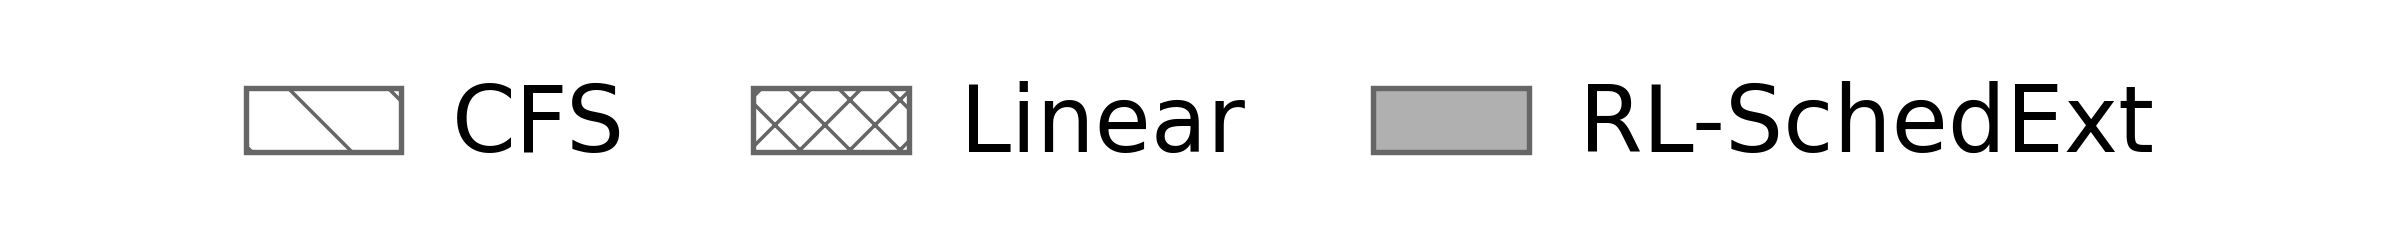
\includegraphics[width=0.50\linewidth]{Figures/fig5_1_legend.png}\par\smallskip
  \captionsetup[subfigure]{font=footnotesize,skip=3pt}
  \begin{subfigure}[b]{0.32\linewidth}
    \centering
    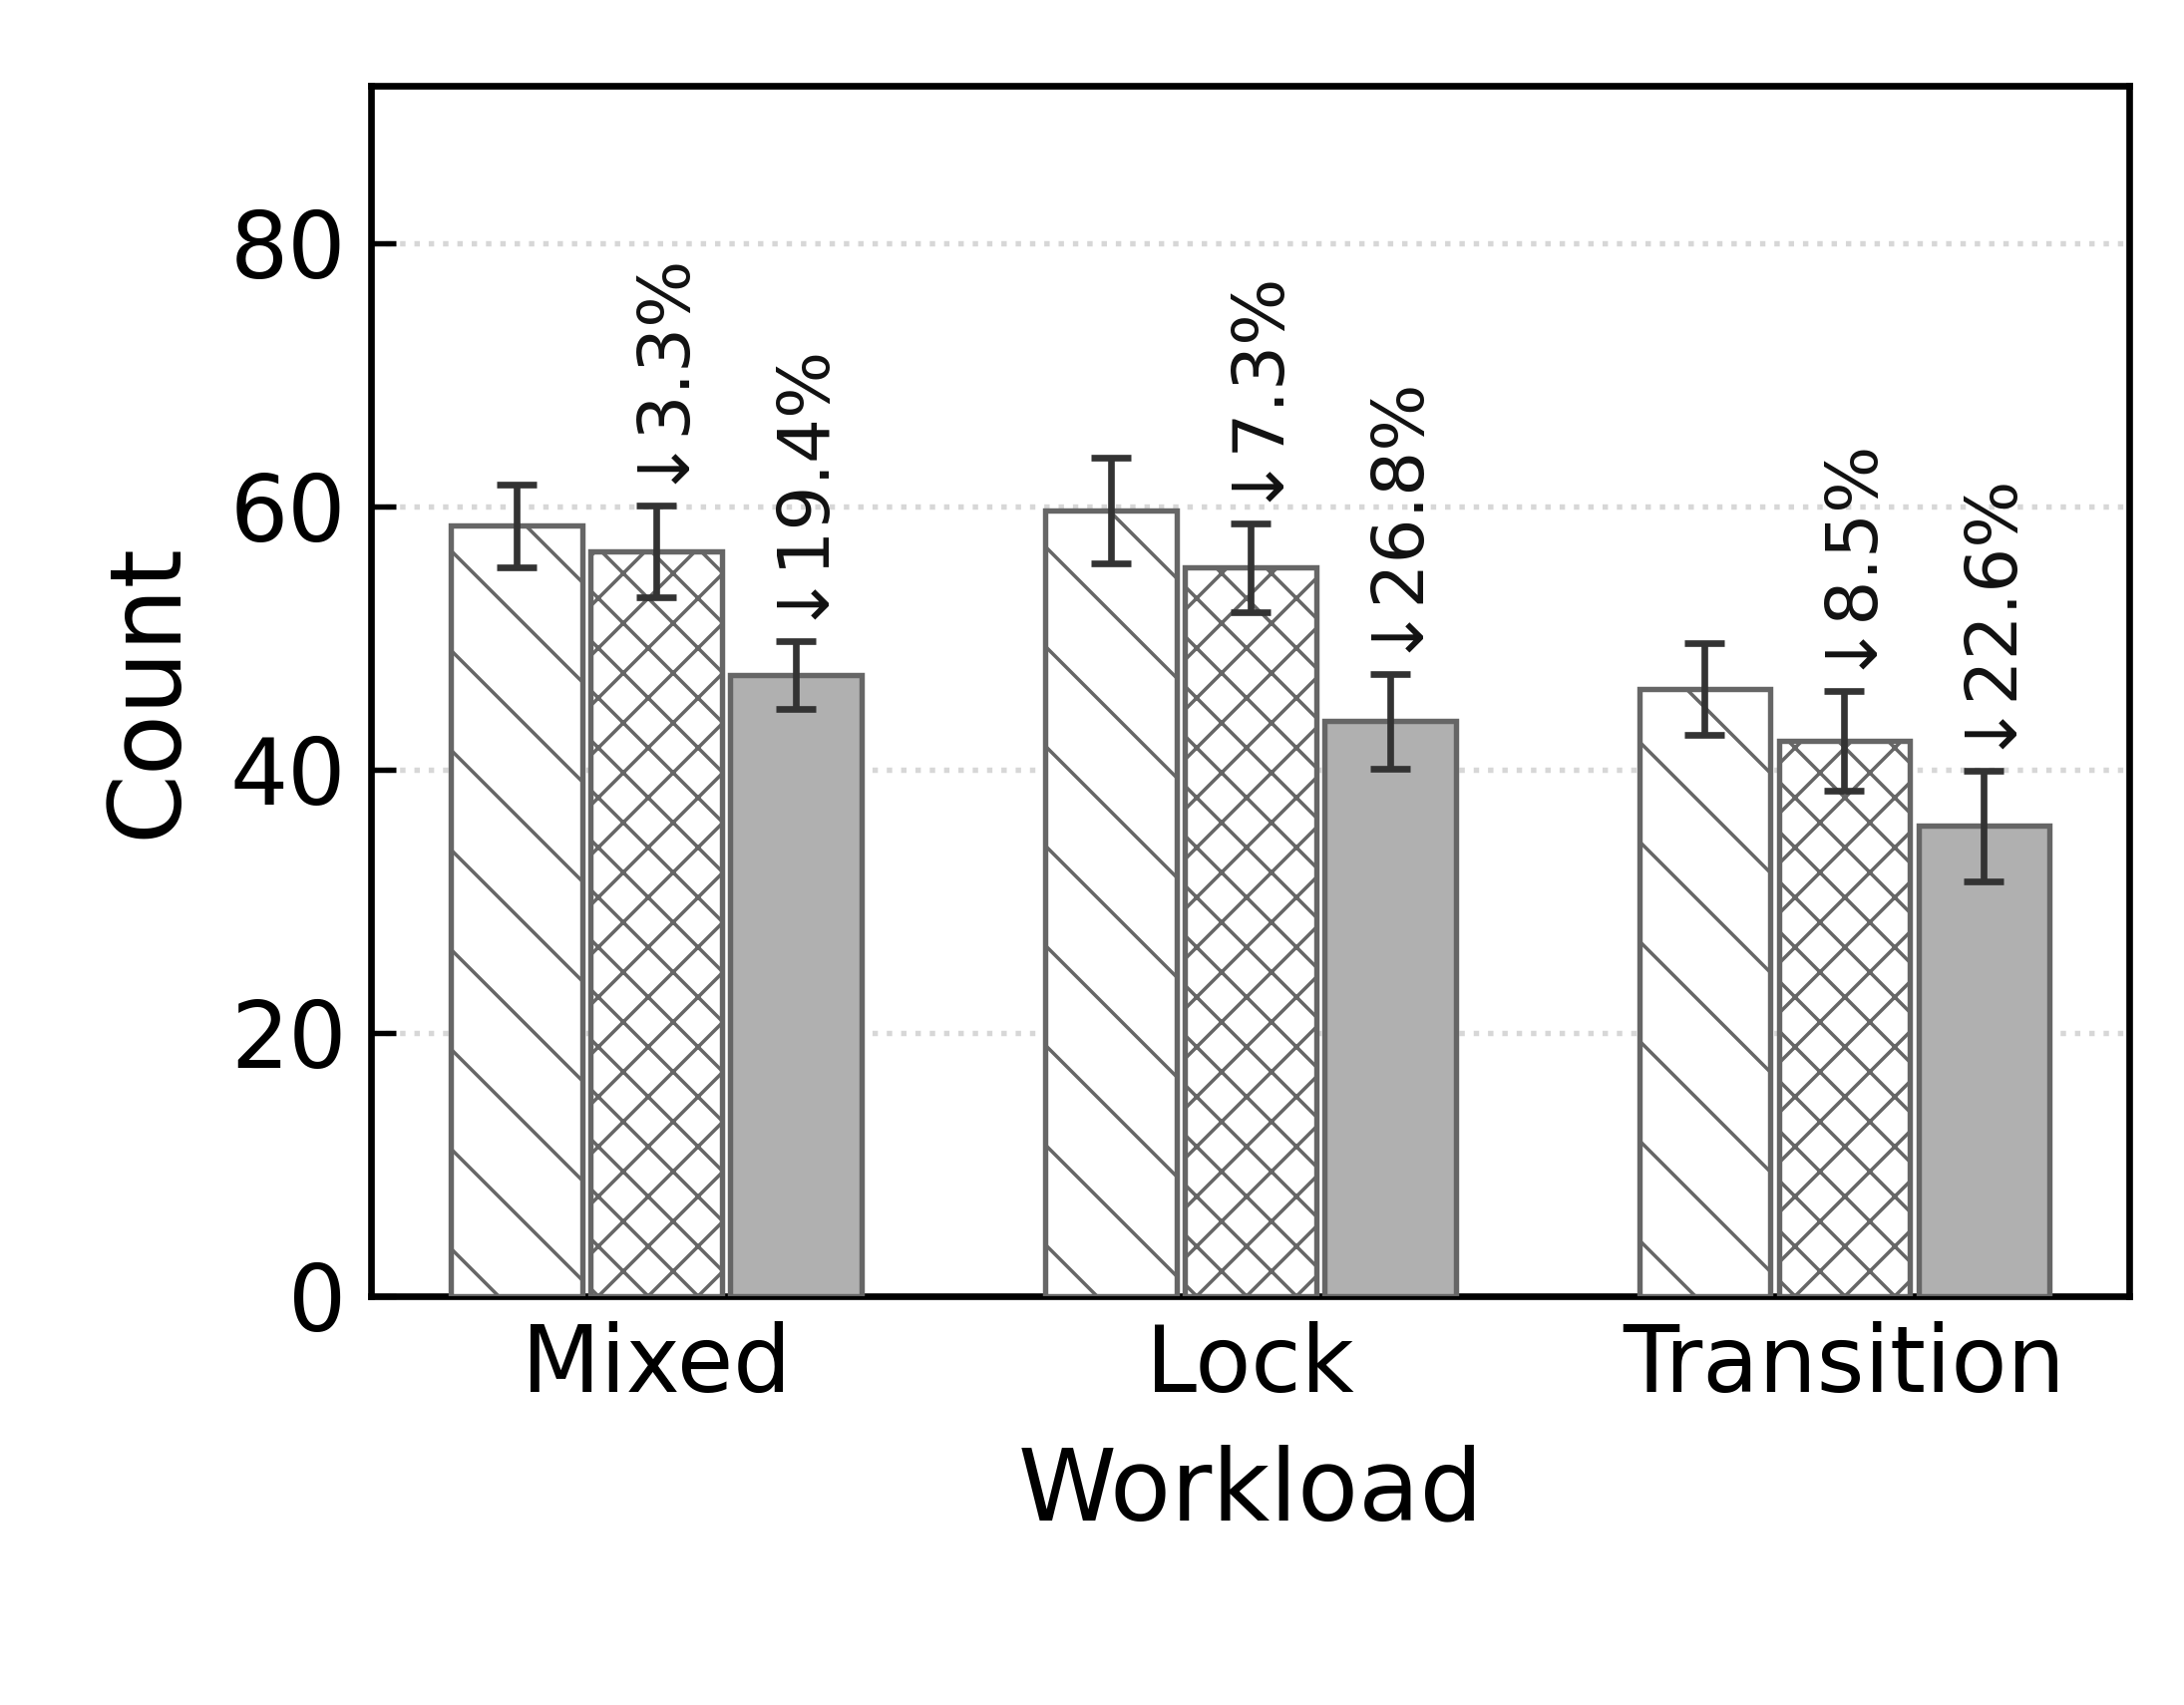
\includegraphics[width=\linewidth]{Figures/fig5_1_a_deadline_miss.png}
    \caption{Deadline miss count}
    \label{fig:sched-deadline}
  \end{subfigure}
  % \hspace{2pt}%
  \begin{subfigure}[b]{0.32\linewidth}
    \centering
    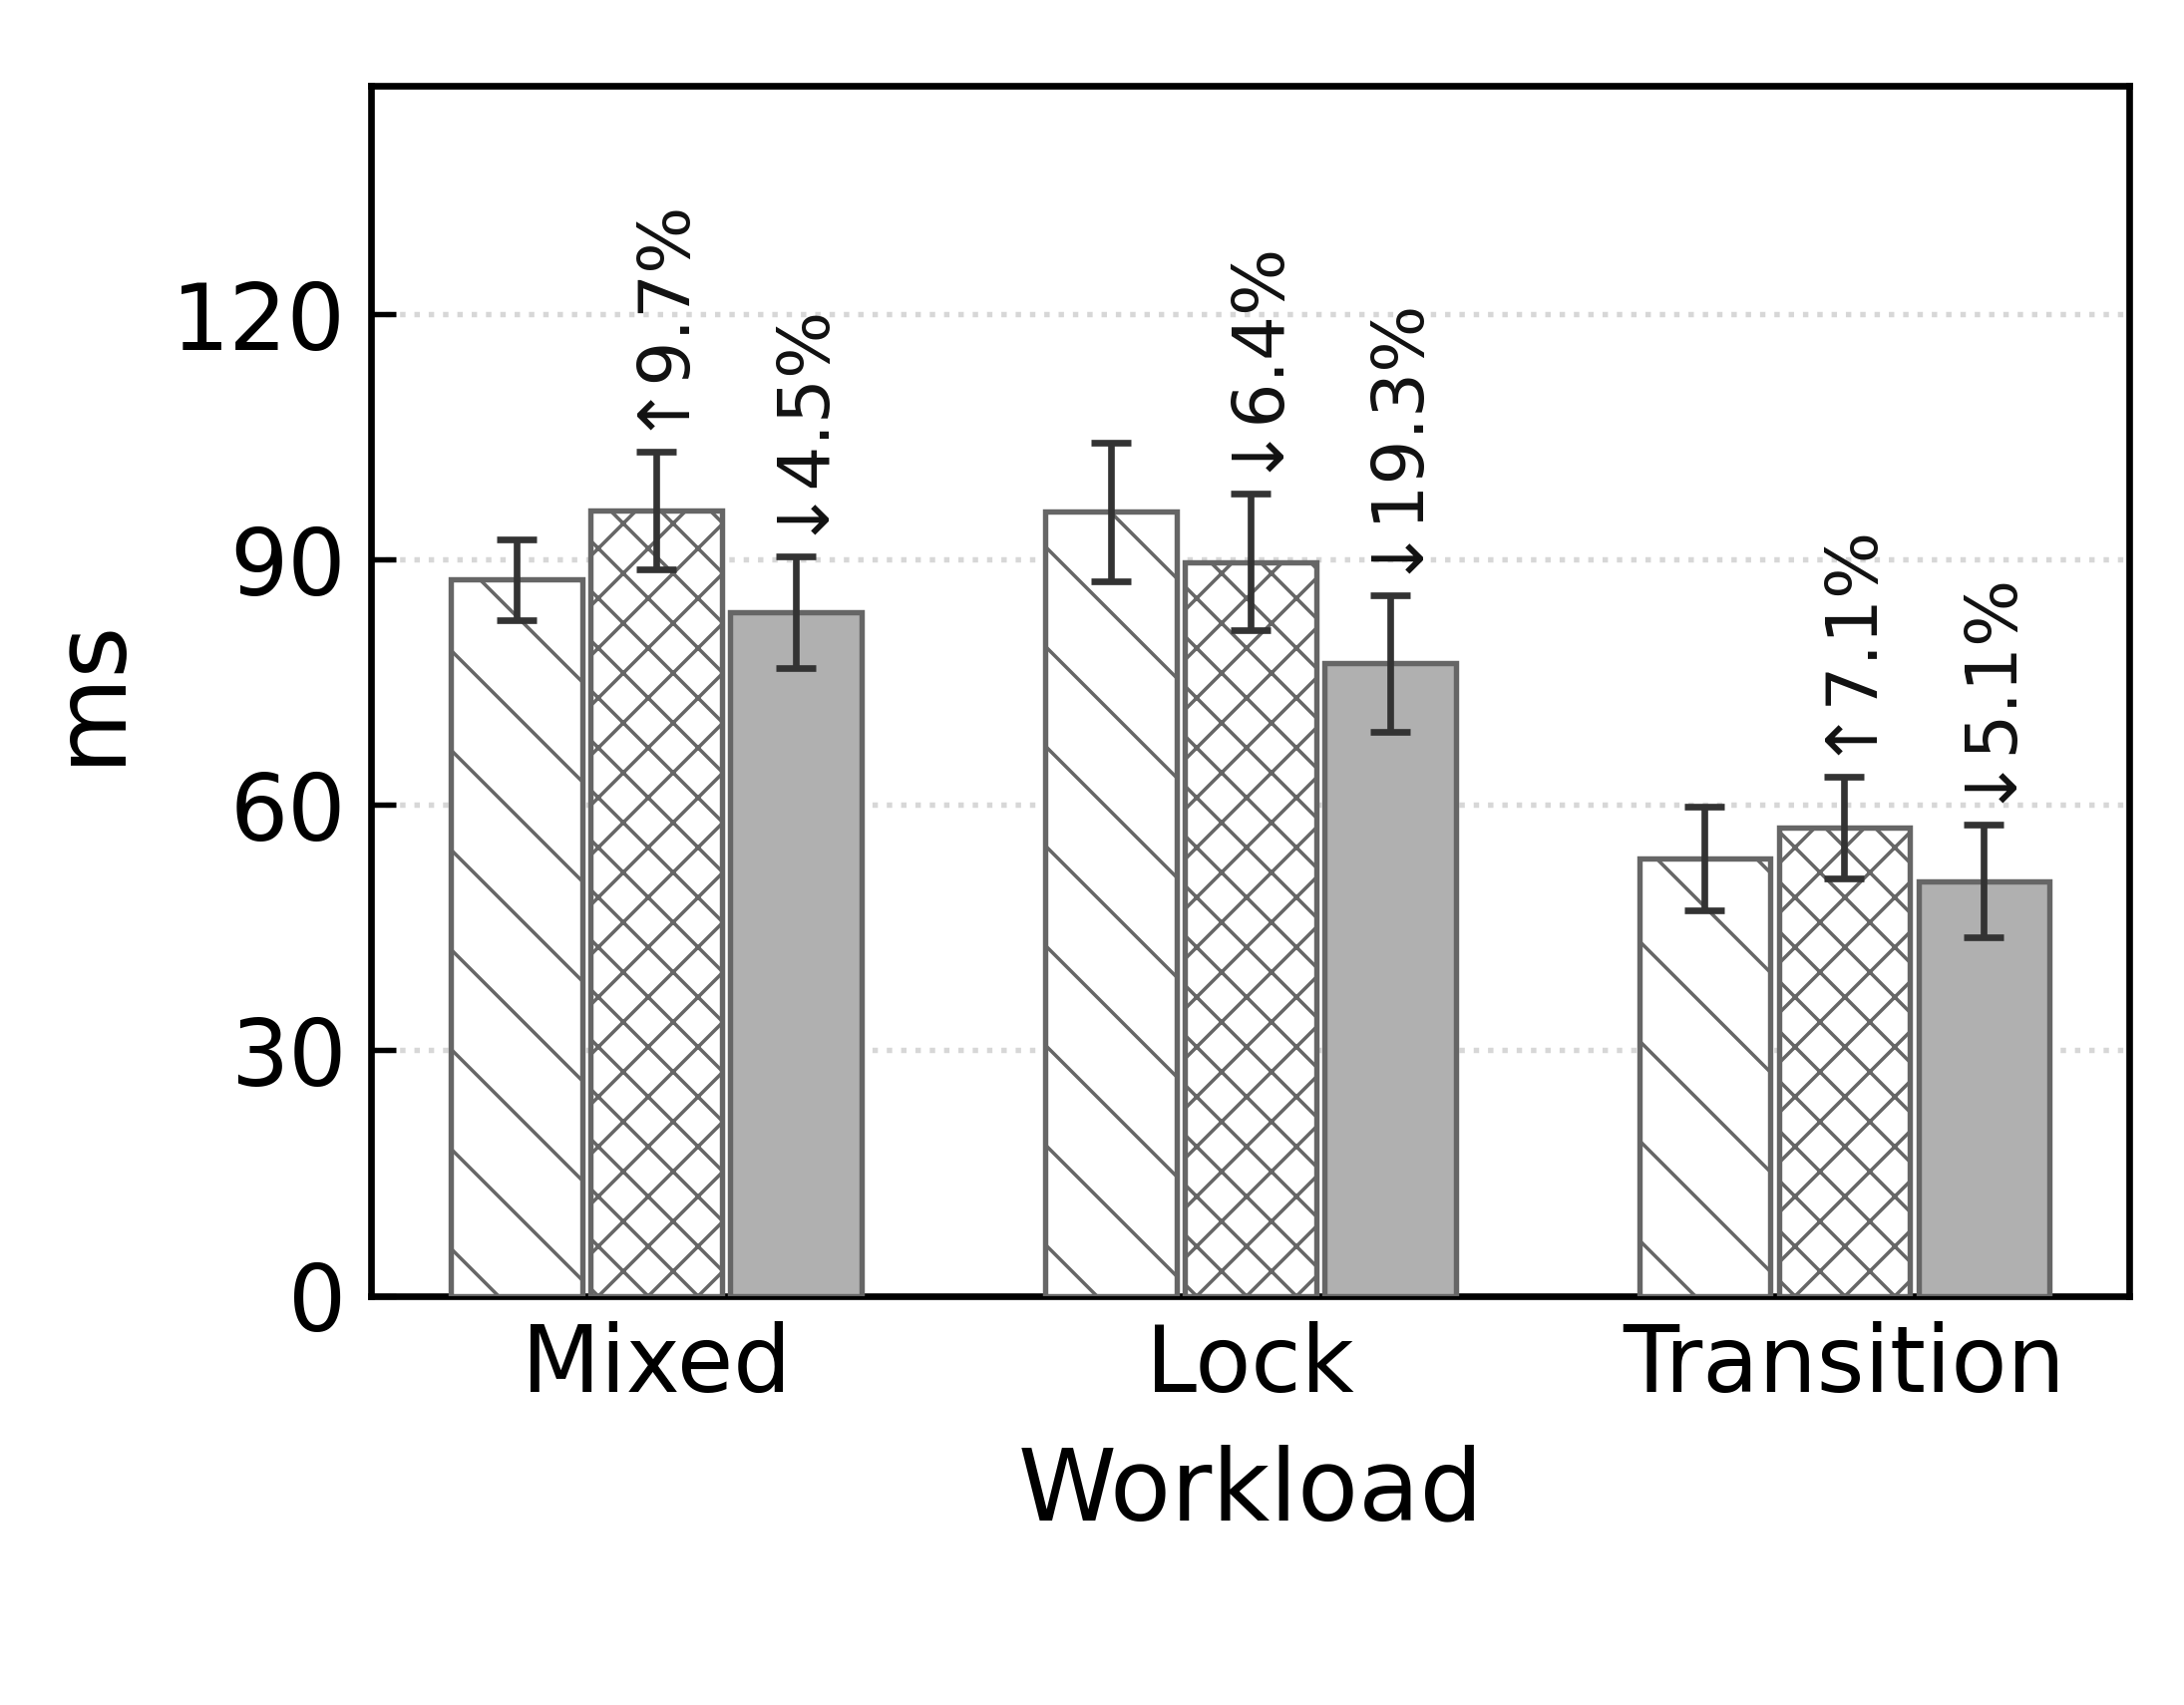
\includegraphics[width=\linewidth]{Figures/fig5_1_b_deadline_overrun.png}
    \caption{Total deadline overrun}
    \label{fig:sched-overrun}
  % \end{subfigure}\par\medskip
    \end{subfigure}
  \begin{subfigure}[b]{0.32\linewidth}
    \centering
    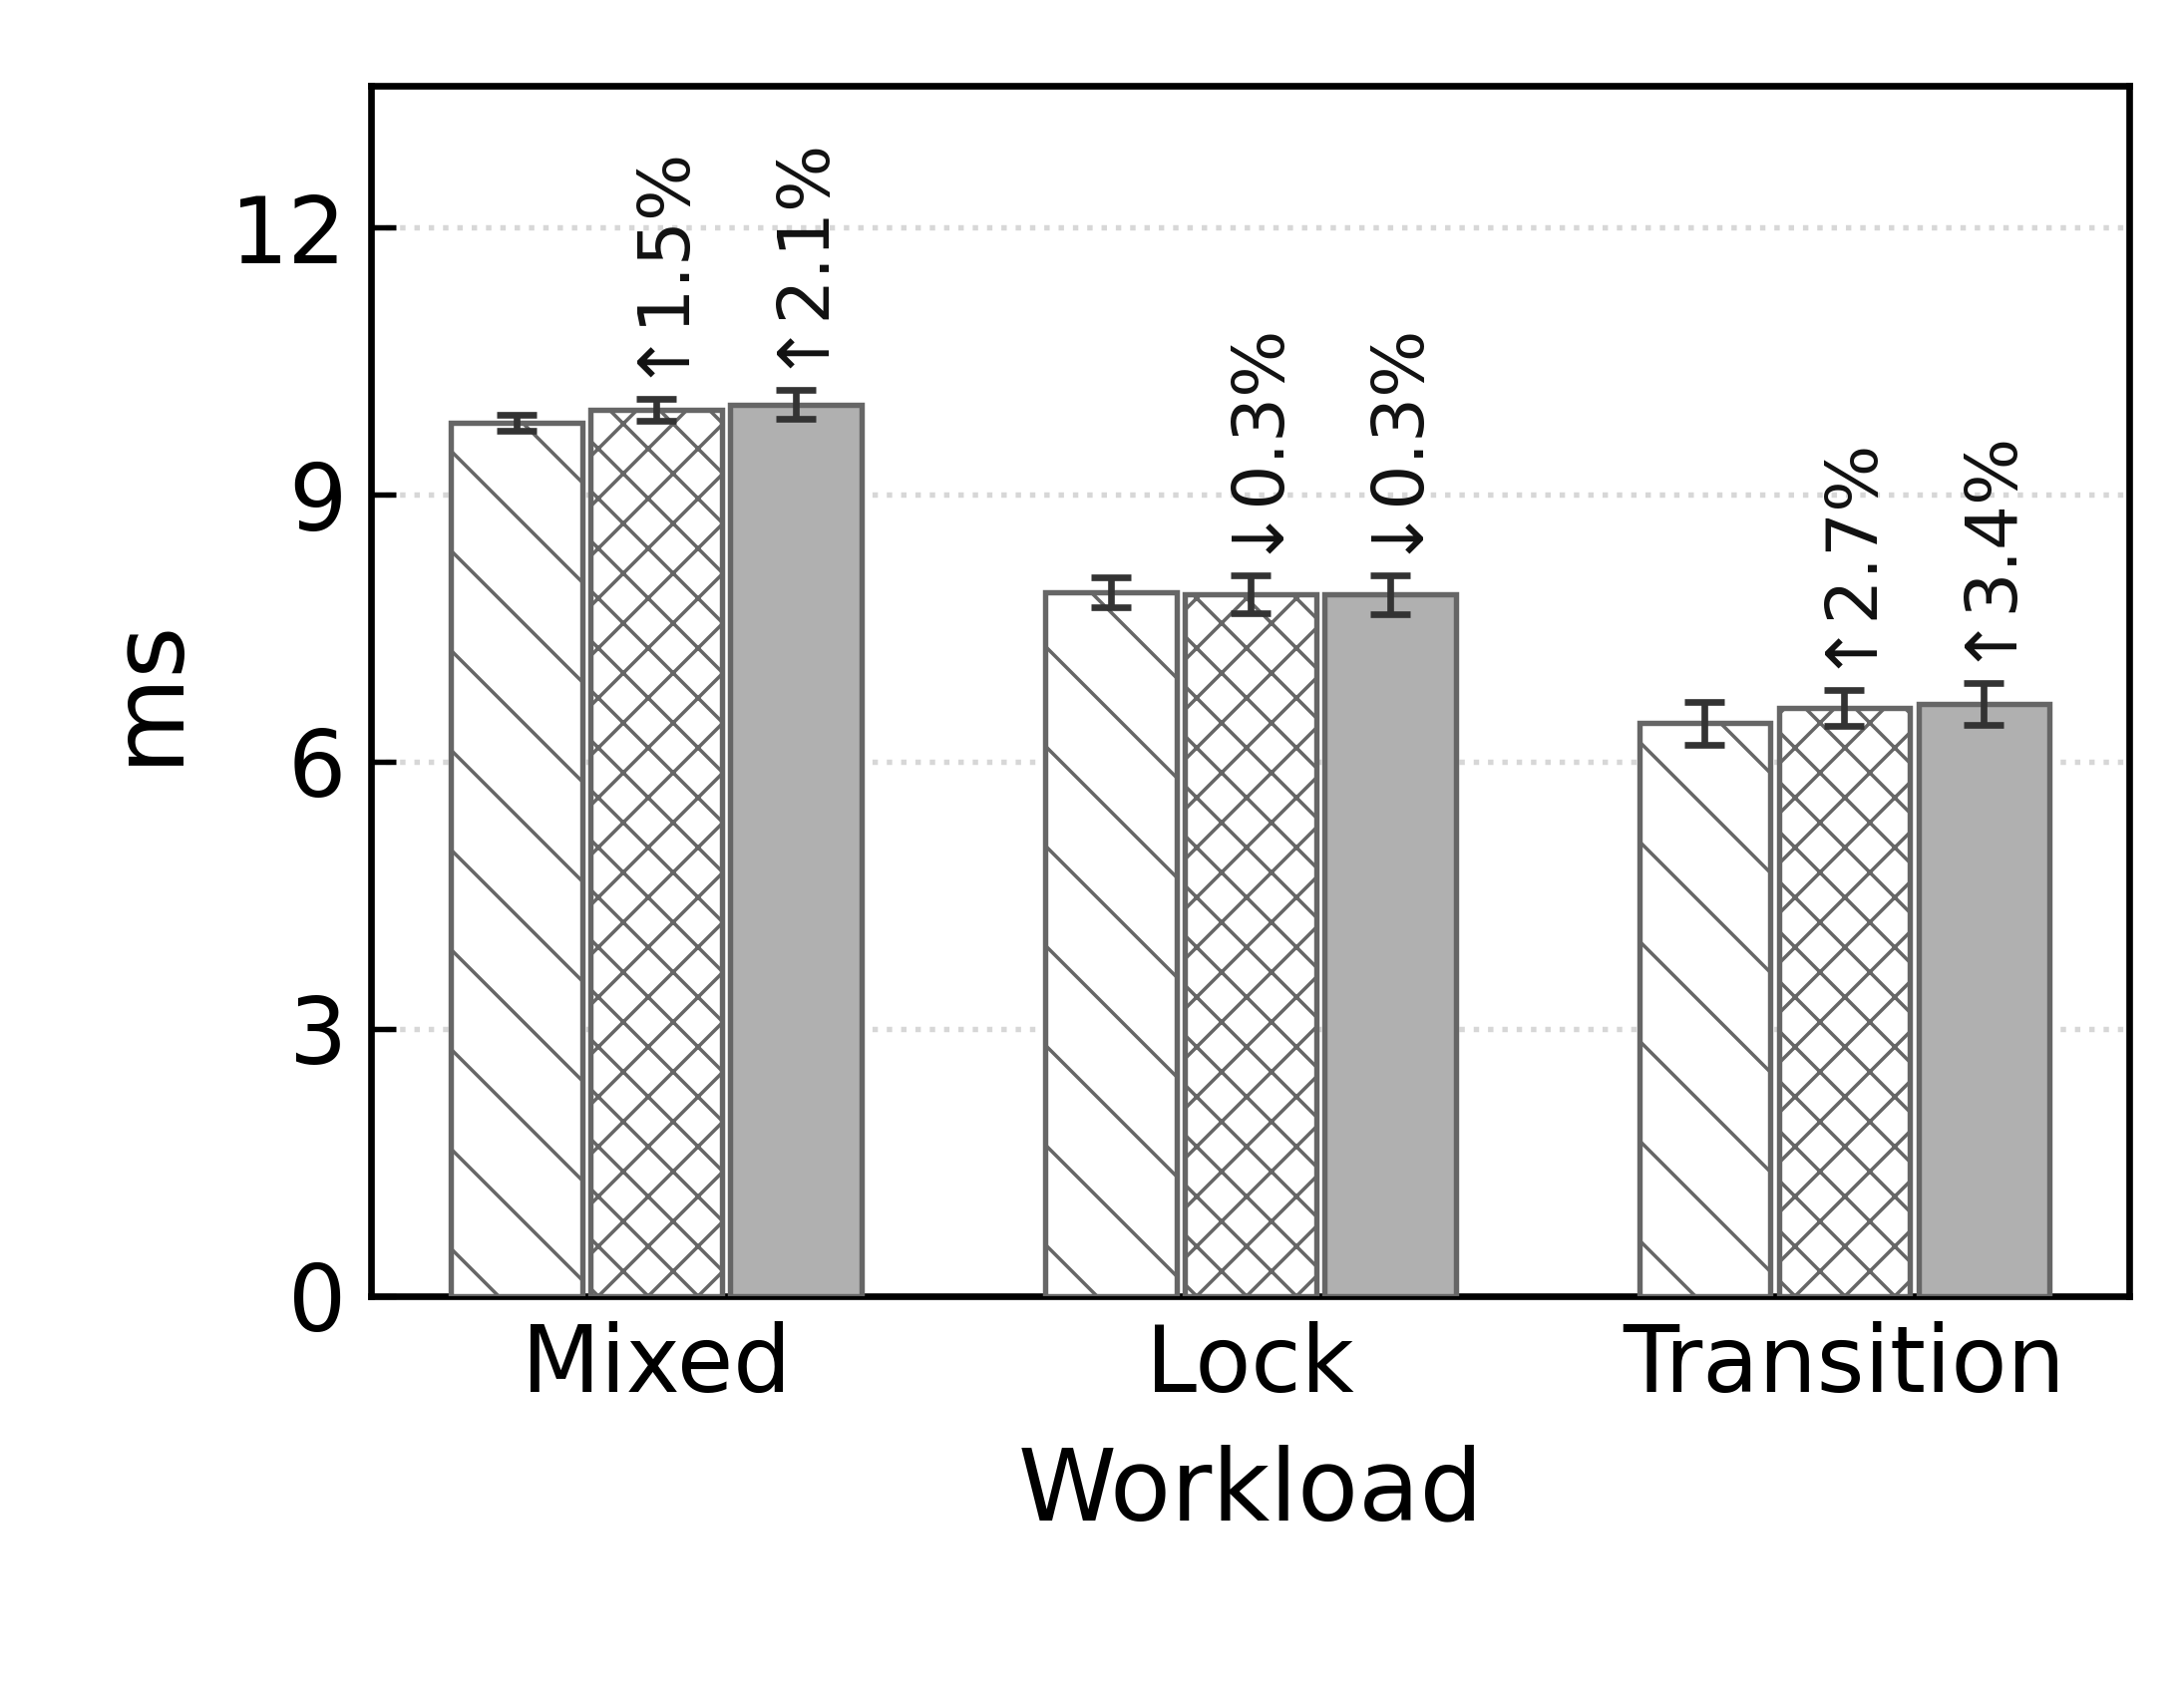
\includegraphics[width=\linewidth]{Figures/fig5_1_c_request_p99.png}
    \caption{Request latency p99}
    \label{fig:sched-p99}
  \end{subfigure}
  \caption{Pixel CPU7에서 수행한 Microbenchmark 결과. (a)--(c)는 Mixed CPU Bursts (Mixed), Lock Dependency (Lock), Workload Transition (Transition)의 성능을 비교한다. 각 지표별로 100회 측정 결과 중 상위 및 하위 5회를 제외한 90회의 결과를 사용하였다. 오차 막대는 표본 표준편차를 나타내며, 화살표는 CFS 대비 변화율을 나타낸다.}
  \label{fig:sched-microbenchmark}
\end{figure}


이러한 결과는 Neural Student가 평가한 세 가지 Workload 모두에서 Linear Student 및 CFS보다 낮은 Deadline Miss Count를 달성했음을 보여준다. 
특히 Mutex를 사용하는 Task 간 의존성이 존재하는 Lock Dependency에서 가장 큰 상대적 개선이 관찰되었다.

\subsection{Deadline Overrun and Tail Latency}
\label{sec:eval-deadline-overrun-and-tail-latency}
Figure~\ref{fig:sched-microbenchmark}(\subref{fig:sched-overrun})은 각 Workload에서 발생한 Total Deadline Overrun을 비교한다. 
Neural Student는 CFS 대비 Mixed CPU Bursts에서 4.5\%, Lock Dependency에서 19.3\%, Workload Transition에서 5.1\%의 Total Deadline Overrun 감소를 기록하였다.

반면 Linear Student는 Mixed CPU Bursts와 Workload Transition에서 각각 9.7\%, 7.1\%의 Total Deadline Overrun 증가를 보였으며, Lock Dependency에서는 6.4\% 감소하였다. 
이러한 결과는 Deadline Miss Count의 감소가 반드시 Total Deadline Overrun의 감소로 이어지는 것은 아님을 보여준다.
즉, Deadline을 놓친 Request의 개수뿐 아니라 개별 Request가 Deadline을 얼마나 초과했는지도 Scheduling Policy의 성능을 평가하는 데 중요한 요소이다.

Figure~\ref{fig:sched-microbenchmark}(\subref{fig:sched-p99})에서 Neural Student의 전체 Request Completion Latency p99는 CFS 대비 Mixed CPU Bursts에서 2.1\%, Workload Transition에서 3.4\% 증가하였으며, Lock Dependency에서는 약 0.3\% 감소하였다. 

Neural Student는 모든 Request의 Completion Latency를 균일하게 줄이기보다는 Scheduling Urgency가 높은 Task를 먼저 실행하도록 Task Ordering을 조정한다. 
그 과정에서 상대적으로 Urgency가 낮은 Task의 CPU 실행 기회가 늦어져 일부 Request의 Completion Latency가 증가할 수 있다. 
이러한 trade-off가 실제 성능에 어떻게 나타나는지 확인하기 위해 다음에서 Deadline Budget별 Request Completion Latency를 분석한다.

\section{Scheduling Policy Analysis}
\label{sec:eval-scheduling-policy-analysis}

\subsection{Latency Redistribution}
\label{sec:eval-latency-redistribution}
앞선 실험에서 Neural Student는 Deadline Compliance를 향상시켰으나,
일부 Workload에서는 전체 Request Completion Latency p99가 증가하였다.
이러한 Latency 증가가 Scheduling Urgency가 높은 Task에서 발생한 것인지,
상대적으로 낮은 Task에서 발생한 것인지 확인하기 위해
Mixed CPU Bursts를 대상으로 추가 분석을 수행하였다.

각 Scheduler에서 측정한 Request Completion Latency를 실험 종료 후
해당 Request의 Deadline Budget과 Mapping하였다.
이를 통해 Deadline Budget에 따라 Request를 분류하고,
각 구간에서 Linear Student와 Neural Student의 p99가
CFS 대비 얼마나 변화하였는지 비교하였다.
실험 결과는 100회 반복의 평균으로 산출하였으며,
오차 막대는 Bootstrap을 이용한 95\% 신뢰구간을 나타낸다~\cite{bootstrap}.

Figure~\ref{fig:bimodal-p99-budget}에서
Deadline Budget이 4\,ms 미만인 Request의 p99는 CFS 대비
Linear Student에서 5.9\% 증가한 반면, Neural Student에서는
25.3\% 감소하였다.
Neural Student는 4--6\,ms 구간에서도 p99를 18.9\% 감소시켰으나,
6--8\,ms 및 8\,ms 이상 구간에서는 각각 0.4\%, 3.7\% 증가하였다.

\begin{figure}[H]
    \centering
    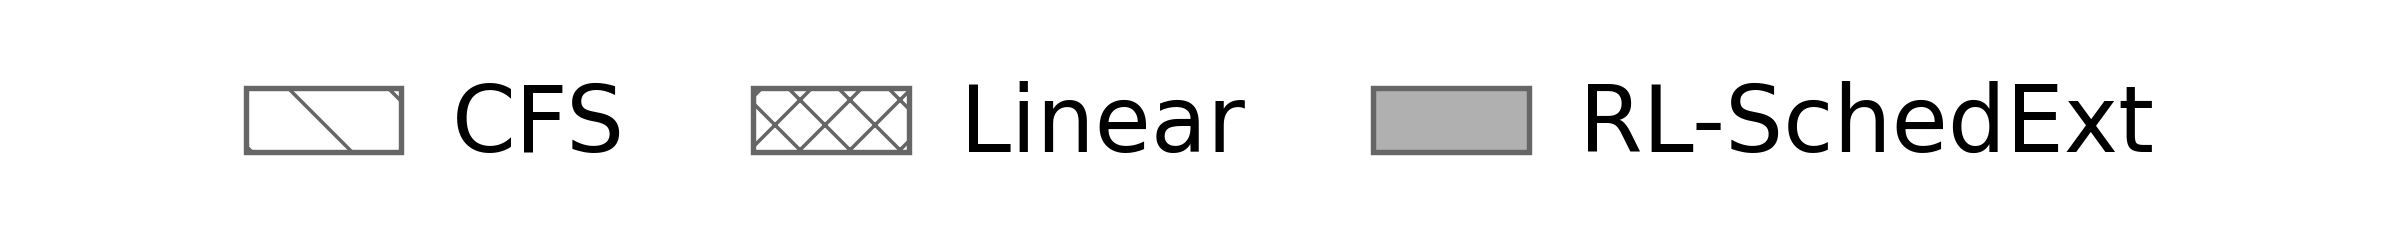
\includegraphics[width=0.50\linewidth]{Figures/fig5_2_legend.png}\par\smallskip
    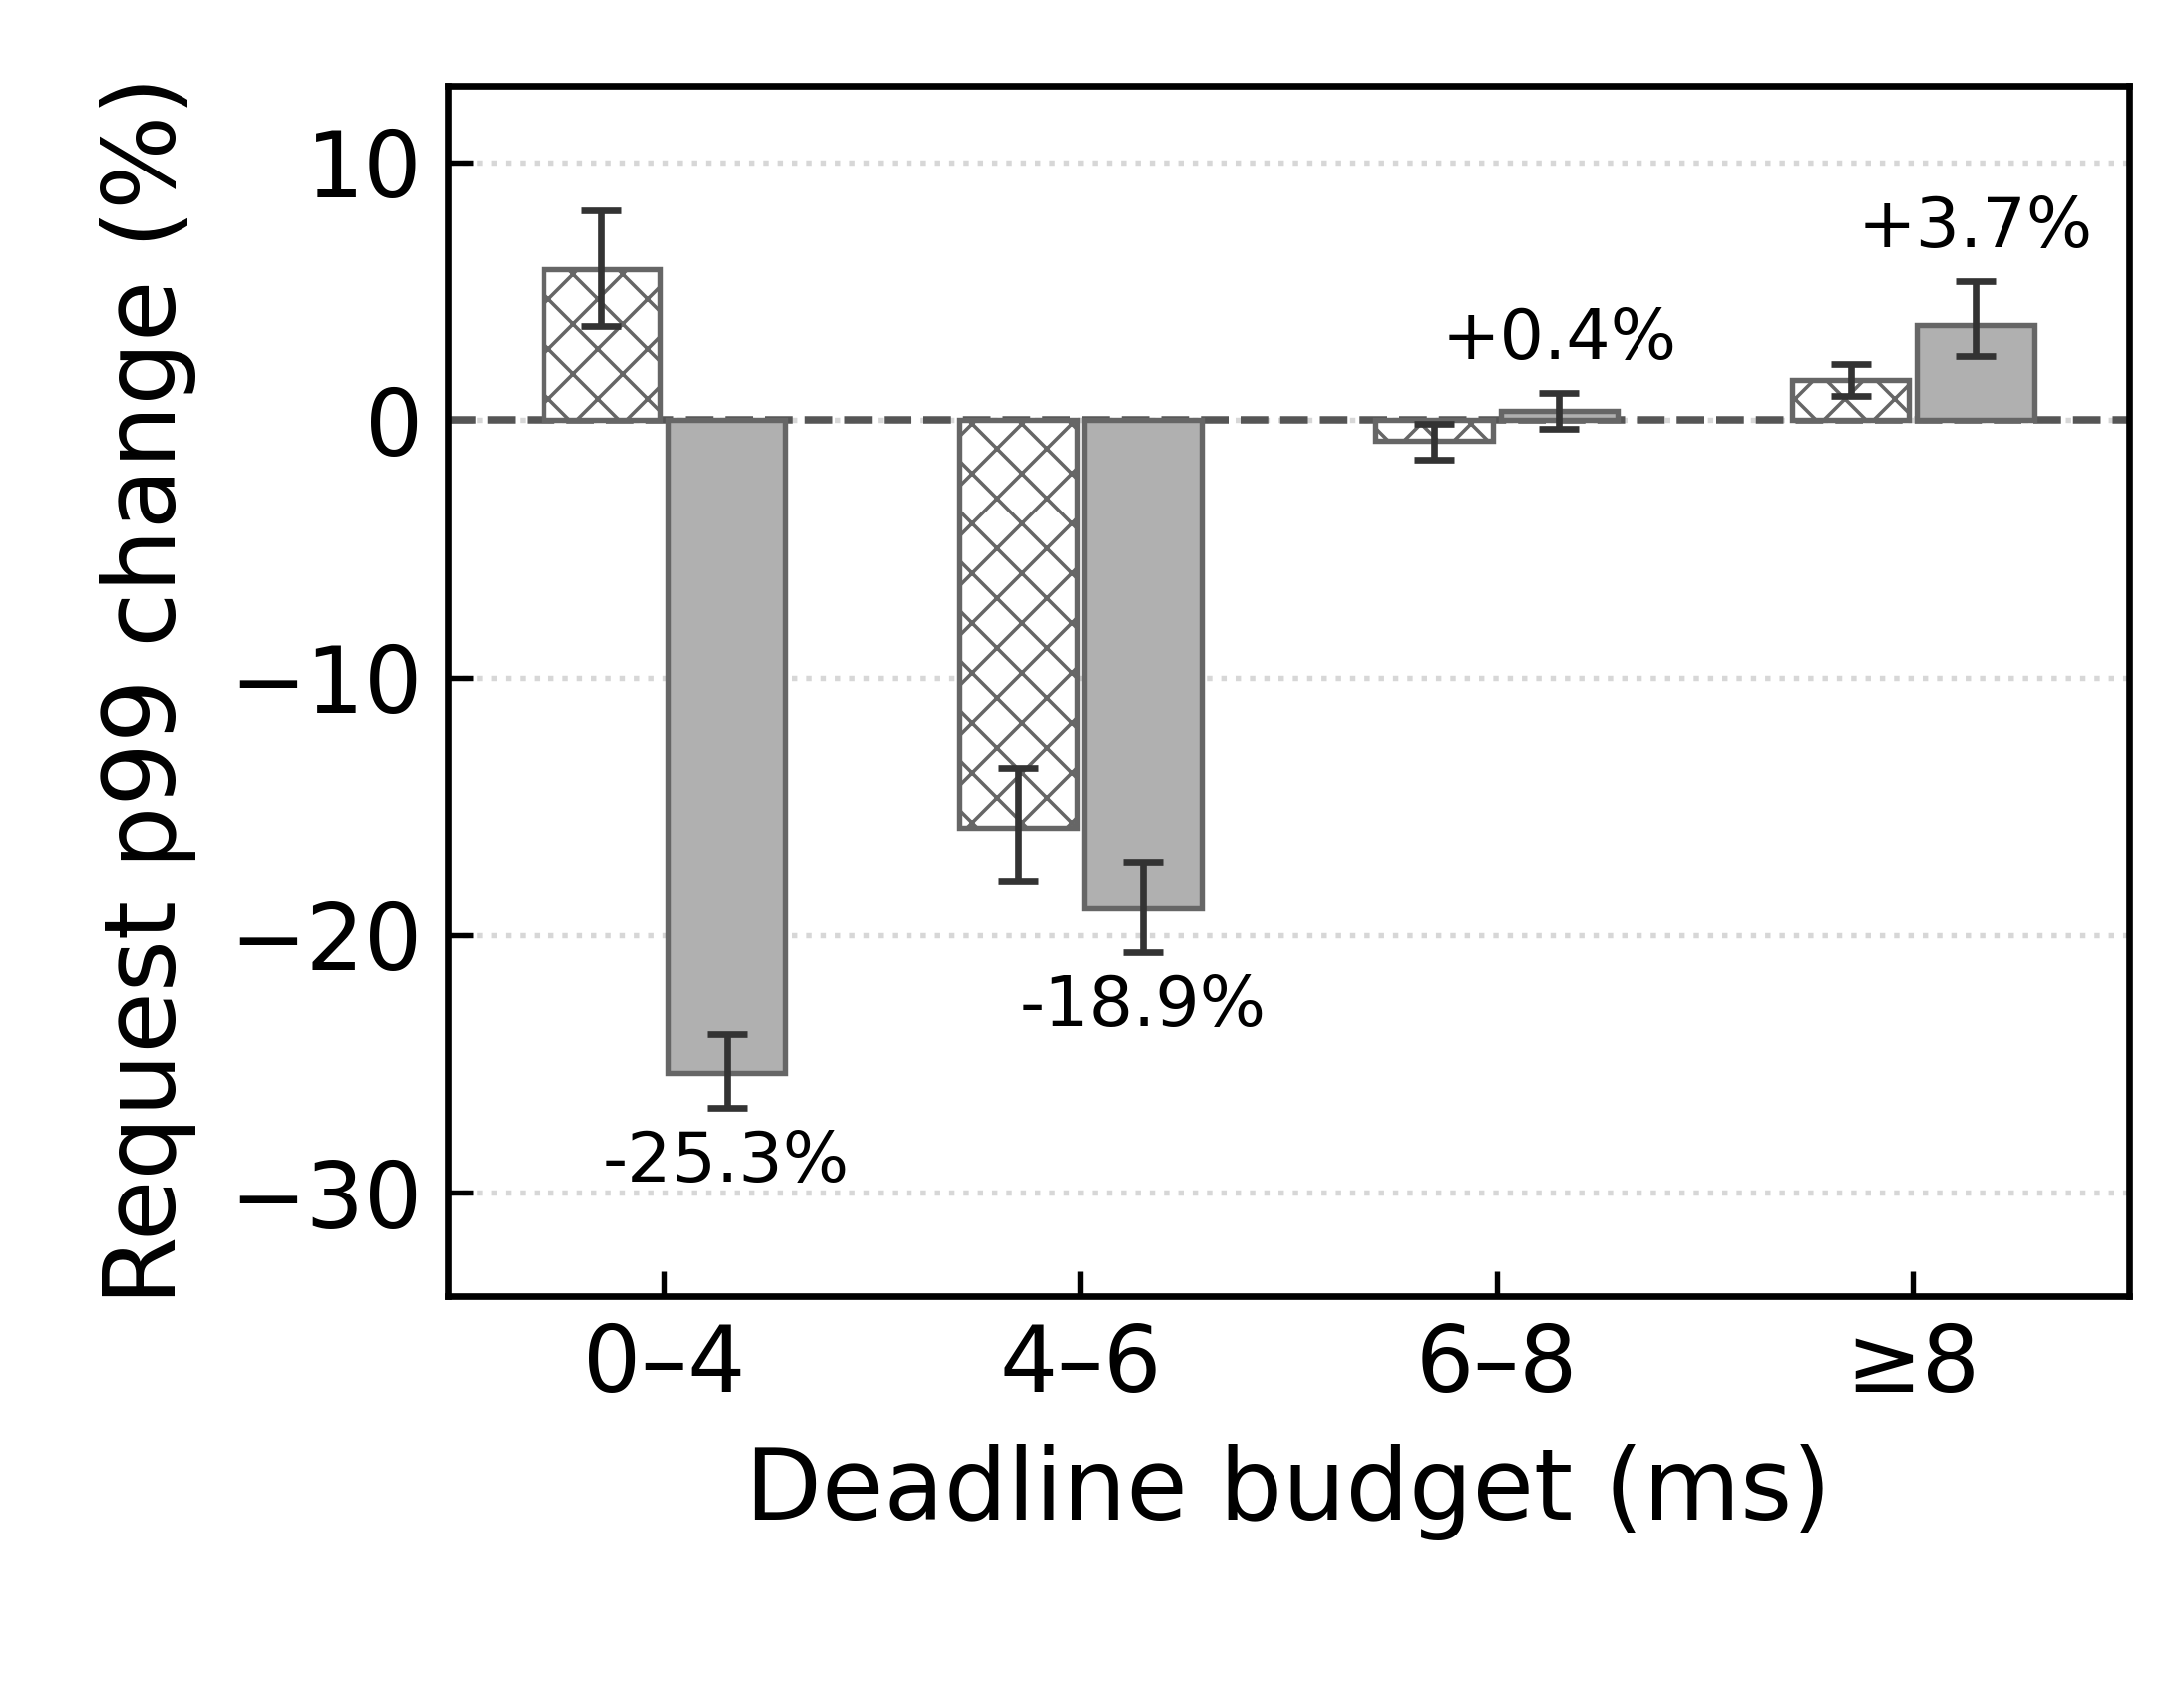
\includegraphics[width=0.65\linewidth]{Figures/fig5_2_mixed_p99_change.png}
    \caption{Mixed CPU Bursts에서 초기 Deadline Budget에 따른 Request Completion Latency p99의 변화율. 전체 100회의 측정 결과를 사용하였다. 점선은 CFS 기준값(0\%)을 나타내며, 오차 막대는 Bootstrap 95\% 신뢰구간을 나타낸다. 음의 변화율은 Latency 감소를 의미한다.}
    \label{fig:bimodal-p99-budget}
\end{figure}

이러한 결과는 Neural Student에서 Deadline Budget이 짧은 Request의
Completion Latency는 감소하는 반면, Deadline Budget이 상대적으로 긴 Request의
Completion Latency는 일부 증가하는 경향을 보여준다.
즉, Neural Student는 전체 Request Completion Latency를 균일하게 감소시키기보다
Scheduling Urgency를 고려하여 Task Ordering을 조정함으로써
Deadline Compliance를 향상시킨다.

\subsection{Analysis of Learned Vruntime Adjustment}
\label{sec:eval-analysis-of-learned-vruntime-adjustment}
앞선 실험에서는 Neural Student가 Linear Student보다 높은
Deadline Compliance를 달성하였다.
이러한 성능 차이를 분석하고 Task Ordering에 비선형 모델이 필요한
이유를 확인하기 위해, 두 Student가 Task의 Scheduling Urgency를
얼마나 효과적으로 구분하는지 평가하였다.

앞선 Microbenchmark와 동일한 Workload를 포함하여 각 Student에 대해
100회의 반복 실험을 수행하였다.
각 Scheduling Decision에서 Student는 관측 가능한 Task의 State를
기반으로 Learned Vruntime Adjustment를 결정한다.
그러나 실제 Scheduling 시점에는 Application Request의 Remaining Deadline을
알 수 없으므로, 각 Decision에서 생성된 Adjustment를 Kernel Trace로
수집하고 실험 종료 후 해당 Task가 처리하던 Request의 실제
Remaining Deadline과 Mapping하였다.

Figure~\ref{fig:deadline-relative-correction}은 실제 Remaining Deadline과
Relative Learned Vruntime Adjustment 사이의 관계를 보여준다.
동일한 Scheduling Decision에서 경쟁하는 Task 간의 상대적인
조정값을 비교하기 위해 각 Task의 Learned Vruntime Adjustment에서
Runnable Task Set의 평균 Learned Vruntime Adjustment를 차감하였다.
Scheduling Decision $k$의 Runnable Task Set을 $\mathcal{R}_k$라 하면,
분석에 사용하는 Relative Learned Vruntime Adjustment는 다음과 같다.

\begin{equation}
    \widetilde{\Delta V}_i =
    \Delta V_i -
    \frac{1}{|\mathcal{R}_k|}
    \sum_{j\in\mathcal{R}_k}\Delta V_j.
    \label{eq:relative_adjustment}
\end{equation}

이 값은 분석을 위해 계산한 값이며 실제 각 Student의 출력이나
Task Selection 방식을 변경하지 않는다.

\begin{figure}[H]
  \centering
  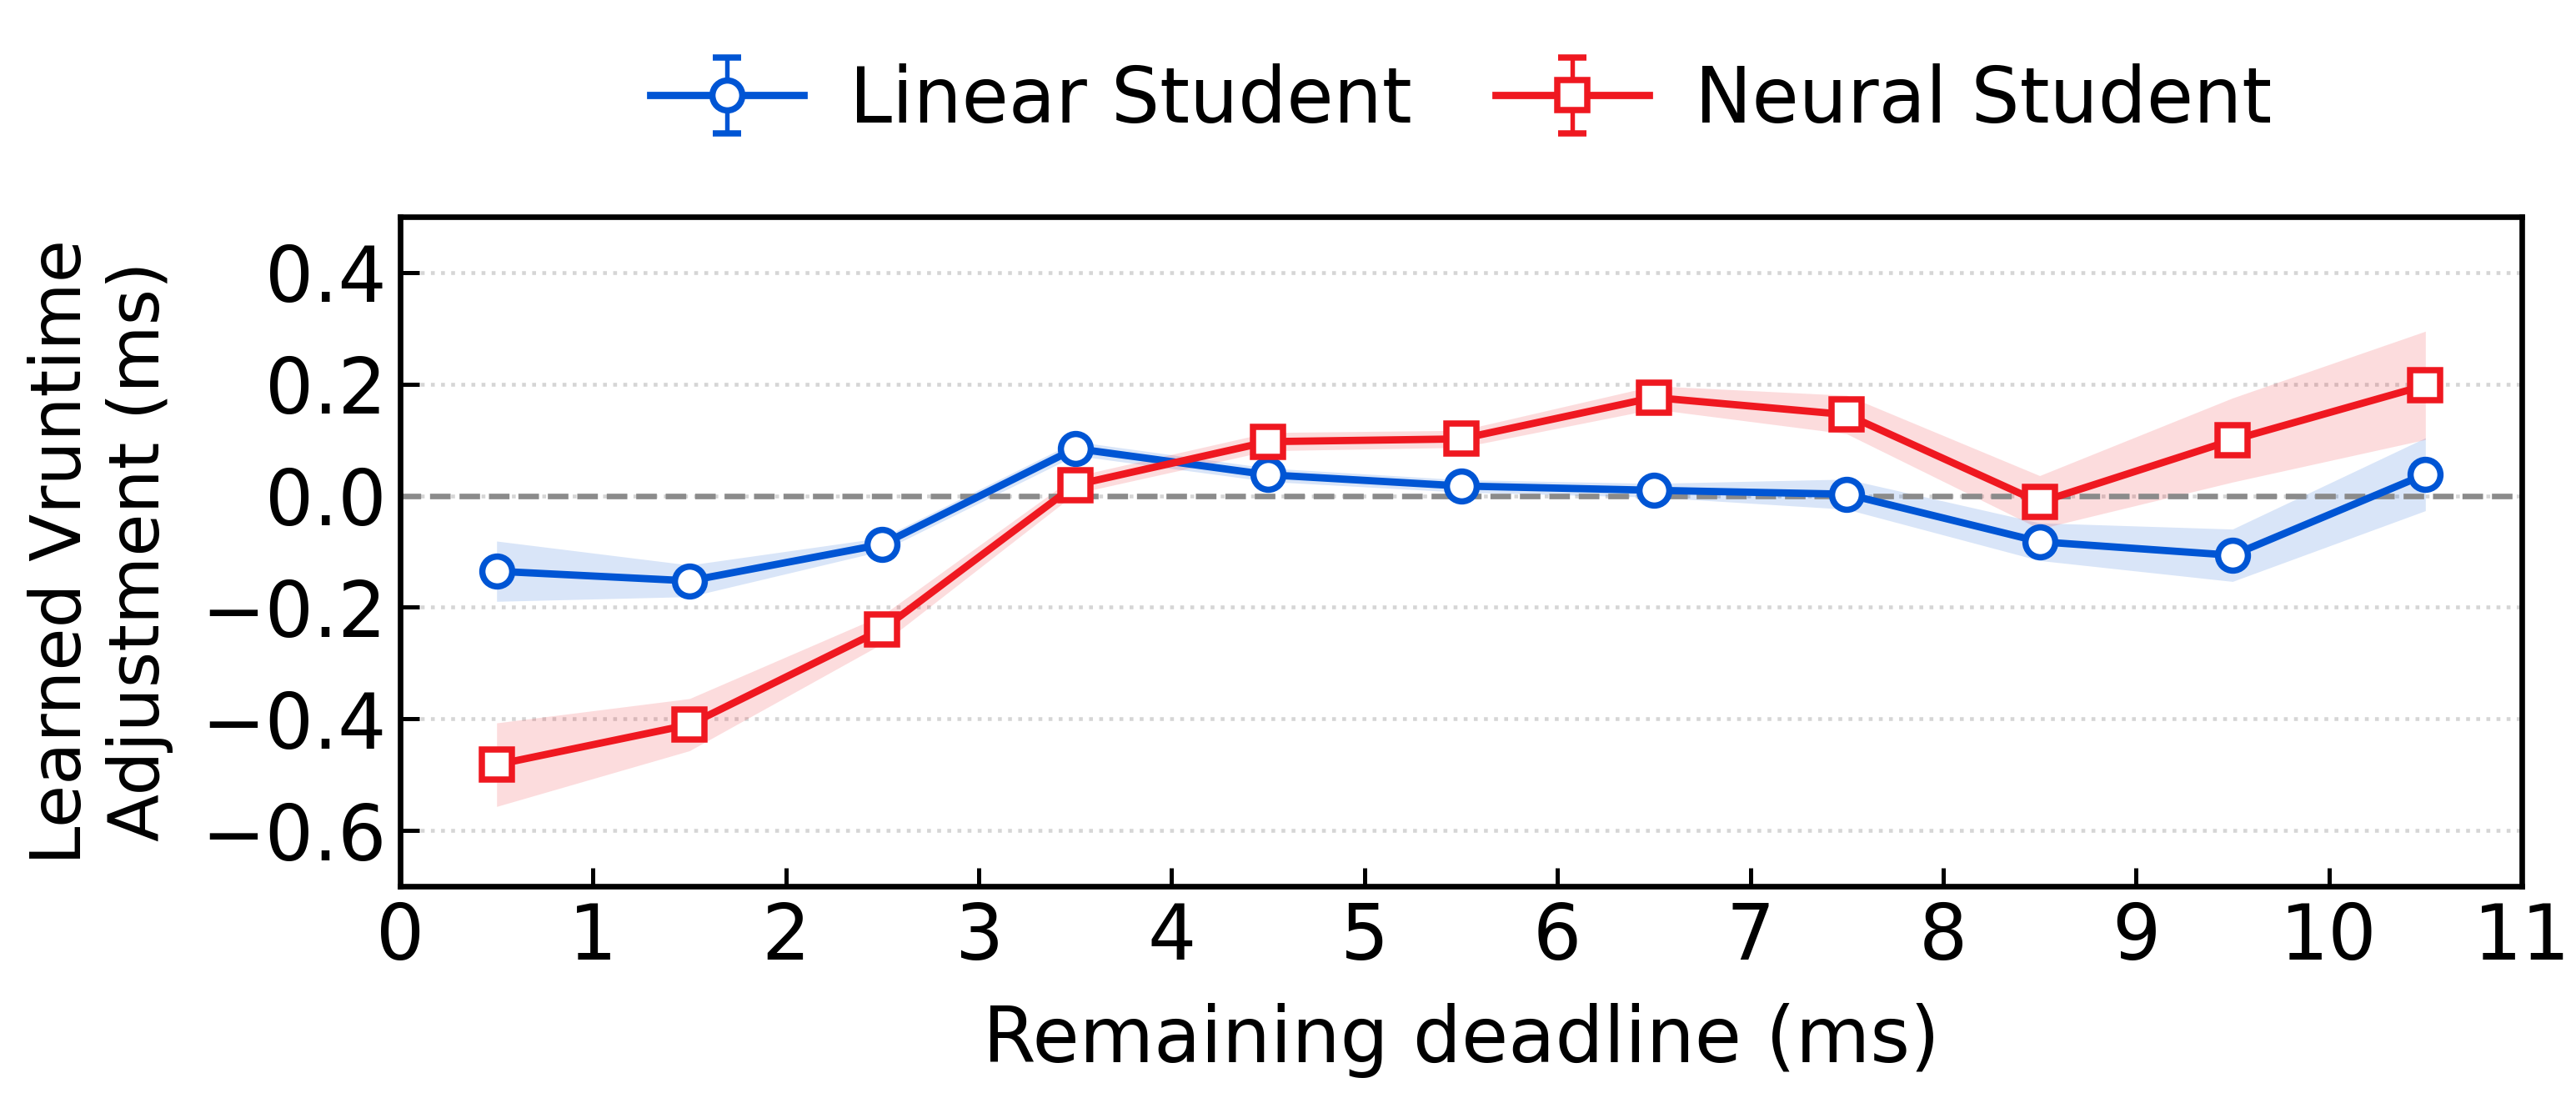
\includegraphics[width=0.82\linewidth]{Figures/fig5_3_deadline_adjustment.png}
  \caption{Remaining Deadline에 따른 Relative Learned Vruntime Adjustment.
  실선은 반복 실험 전체의 평균, 음영은 평균 $\pm$ 1 Standard Deviation,
  오차 막대는 95\% 신뢰구간을 나타낸다.}
  \label{fig:deadline-relative-correction}
\end{figure}

Neural Student의 Relative Learned Vruntime Adjustment는 처리 중인 Request의
Remaining Deadline이 0--1\,ms인 Task에서 평균 $-0.482$\,ms였으며,
6--7\,ms인 Task에서는 평균 $+0.176$\,ms였다.
두 구간의 Relative Learned Vruntime Adjustment 차이는 0.658\,ms로,
Linear Student의 0.145\,ms보다 약 4.5배 크게 나타났다.
이는 Neural Student가 Remaining Deadline이 짧은 Request를 처리하는 Task와
상대적으로 Remaining Deadline이 긴 Request를 처리하는 Task 사이에
더 큰 Relative Learned Vruntime Adjustment 차이를 보였음을 나타낸다.
이러한 결과는 실제 Deadline 정보가 제공되지 않는 환경에서
Neural Student가 관측 가능한 State로부터 Task의 Scheduling
Urgency를 Linear Student보다 효과적으로 추론함을 보여준다.
따라서 RL Teacher가 학습한 Context-dependent Task Ordering
특성을 유지하기 위해서는 단순한 선형 모델보다
비선형 모델을 사용하는 것이 효과적이다.

\section{Macrobenchmark}
\label{sec:eval-macrobenchmark}
\subsection{Workload and Methodology}
\label{sec:eval-workload-and-methodology}
실제 Android Application에서의 End-to-End 성능을 평가하기 위해 오픈소스 게임 \textit{Mindustry}를 단독으로 실행하였다~\cite{mindustry}. Mindustry는 게임 로직 처리와 렌더링이 동시에 수행되는 Android 게임으로, 게임 진행 상태와 사용자 조작에 따라 CPU 부하가 달라질 수 있다.

따라서 본 연구에서는 Scheduler 간 비교에서 Workload의 변동성을 최소화하기 위해 사전에 구성된 게임 저장 파일을 활용하였다. 60초 동안 Defense를 하는 시나리오를 수행하였으며, 게임의 시뮬레이션과 화면 갱신이 지속적으로 수행된다.

실험 결과는 60초 Defense 구간에서 수집한 SurfaceFlinger TimeStats를 이용하여 Average FPS와 Frame Interval Percentiles (p50, p95, p99)를 비교하였다. Average FPS는 단위 시간당 화면에 표시되는 프레임 수로, 게임의 전반적인 시각적 부드러움을 나타낸다. Frame Interval은 연속된 프레임의 실제 출력 시각 사이의 간격이며, 큰 Frame Interval은 간헐적인 화면 끊김과 Frame Pacing 불안정성을 나타낸다~\cite{timestats,framepacing}.
Mindustry와 같이 게임 로직과 렌더링이 지속적으로 수행되는 환경에서는 Average FPS가 유사하더라도 일부 프레임의 출력이 크게 지연되면 시각적 부드러움이 저하될 수 있다. 따라서 Average FPS뿐 아니라 Frame Interval의 Tail Latency를 함께 비교하여 일반적인 출력 성능과 긴 프레임 지연을 구분해 평가하였다.

실험은 CFS와 RL-SchedExt에 대해 각각 10회씩, 총 20회 반복하여 수행하였다. 매 실행마다 Application을 재시작함으로써 이전 실행에서 유지될 수 있는 게임 내부 상태의 영향을 최소화하고자 하였다. 최종 Average FPS와 Frame Interval은 각 Scheduler에서 측정한 10회 결과의 산술평균으로 산출하였다.


\subsection{Gaming Performance}
\label{sec:eval-gaming-performance}
Figure~\ref{fig:mindustry-macro}는 Mindustry 실행 환경에서 CFS와 RL-SchedExt의 Average FPS 및 Frame Interval을 비교한 결과이다. RL-SchedExt는 Average FPS 29.62를 기록하여 CFS의 26.47 대비 11.9\% 높은 성능을 보였다. 이는 동일한 게임 시나리오에서 단위 시간당 더 많은 프레임을 출력함으로써 게임의 전반적인 화면 갱신 성능을 향상시켰음을 의미한다.

\begin{figure}[H]
  \centering
  
\includegraphics[width=0.40\linewidth]{Figures/fig5_4_legend.png}\par\smallskip
  \captionsetup[subfigure]{skip=2pt}
  \begin{subfigure}[b]{0.39\linewidth}
    \centering
    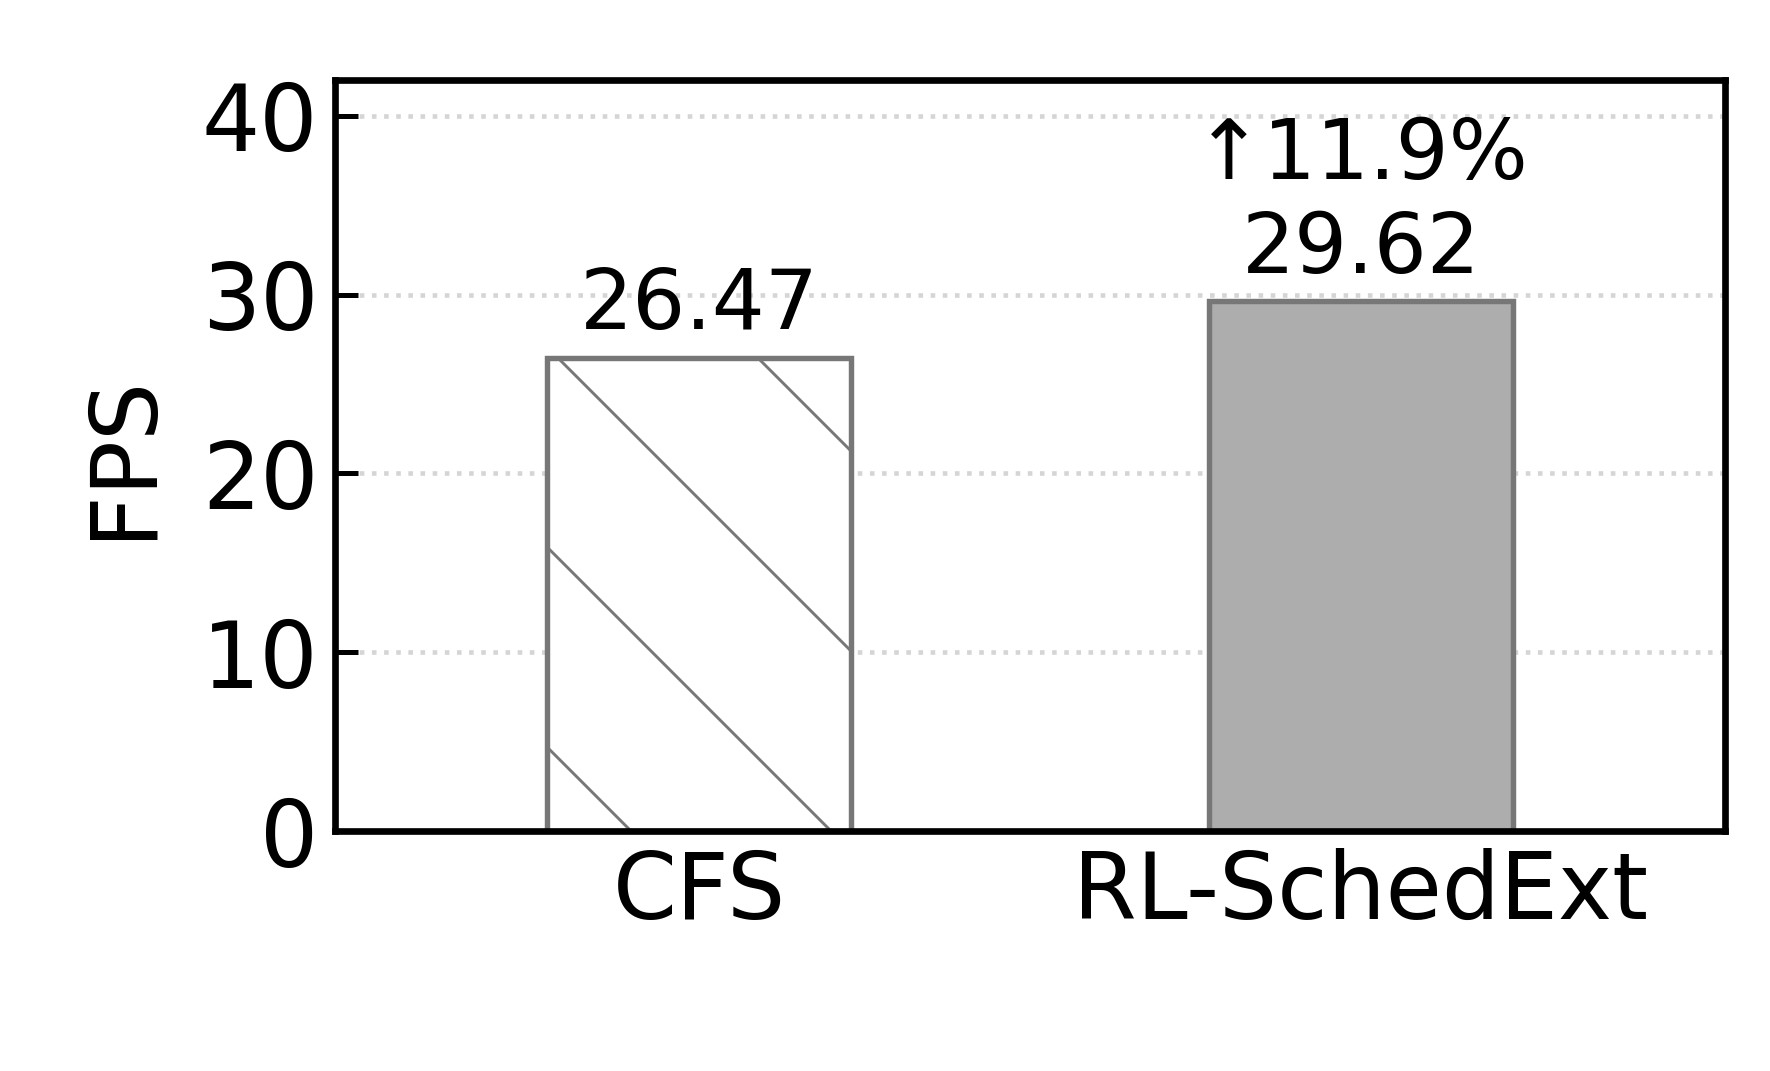
\includegraphics[width=\linewidth]{Figures/fig5_4_a_average_fps.png}
    \subcaption{Average FPS ($\uparrow$)}
    \label{fig:mindustry-fps}
  \end{subfigure}
  \hspace{2pt}%
  \begin{subfigure}[b]{0.575\linewidth}
    \centering
    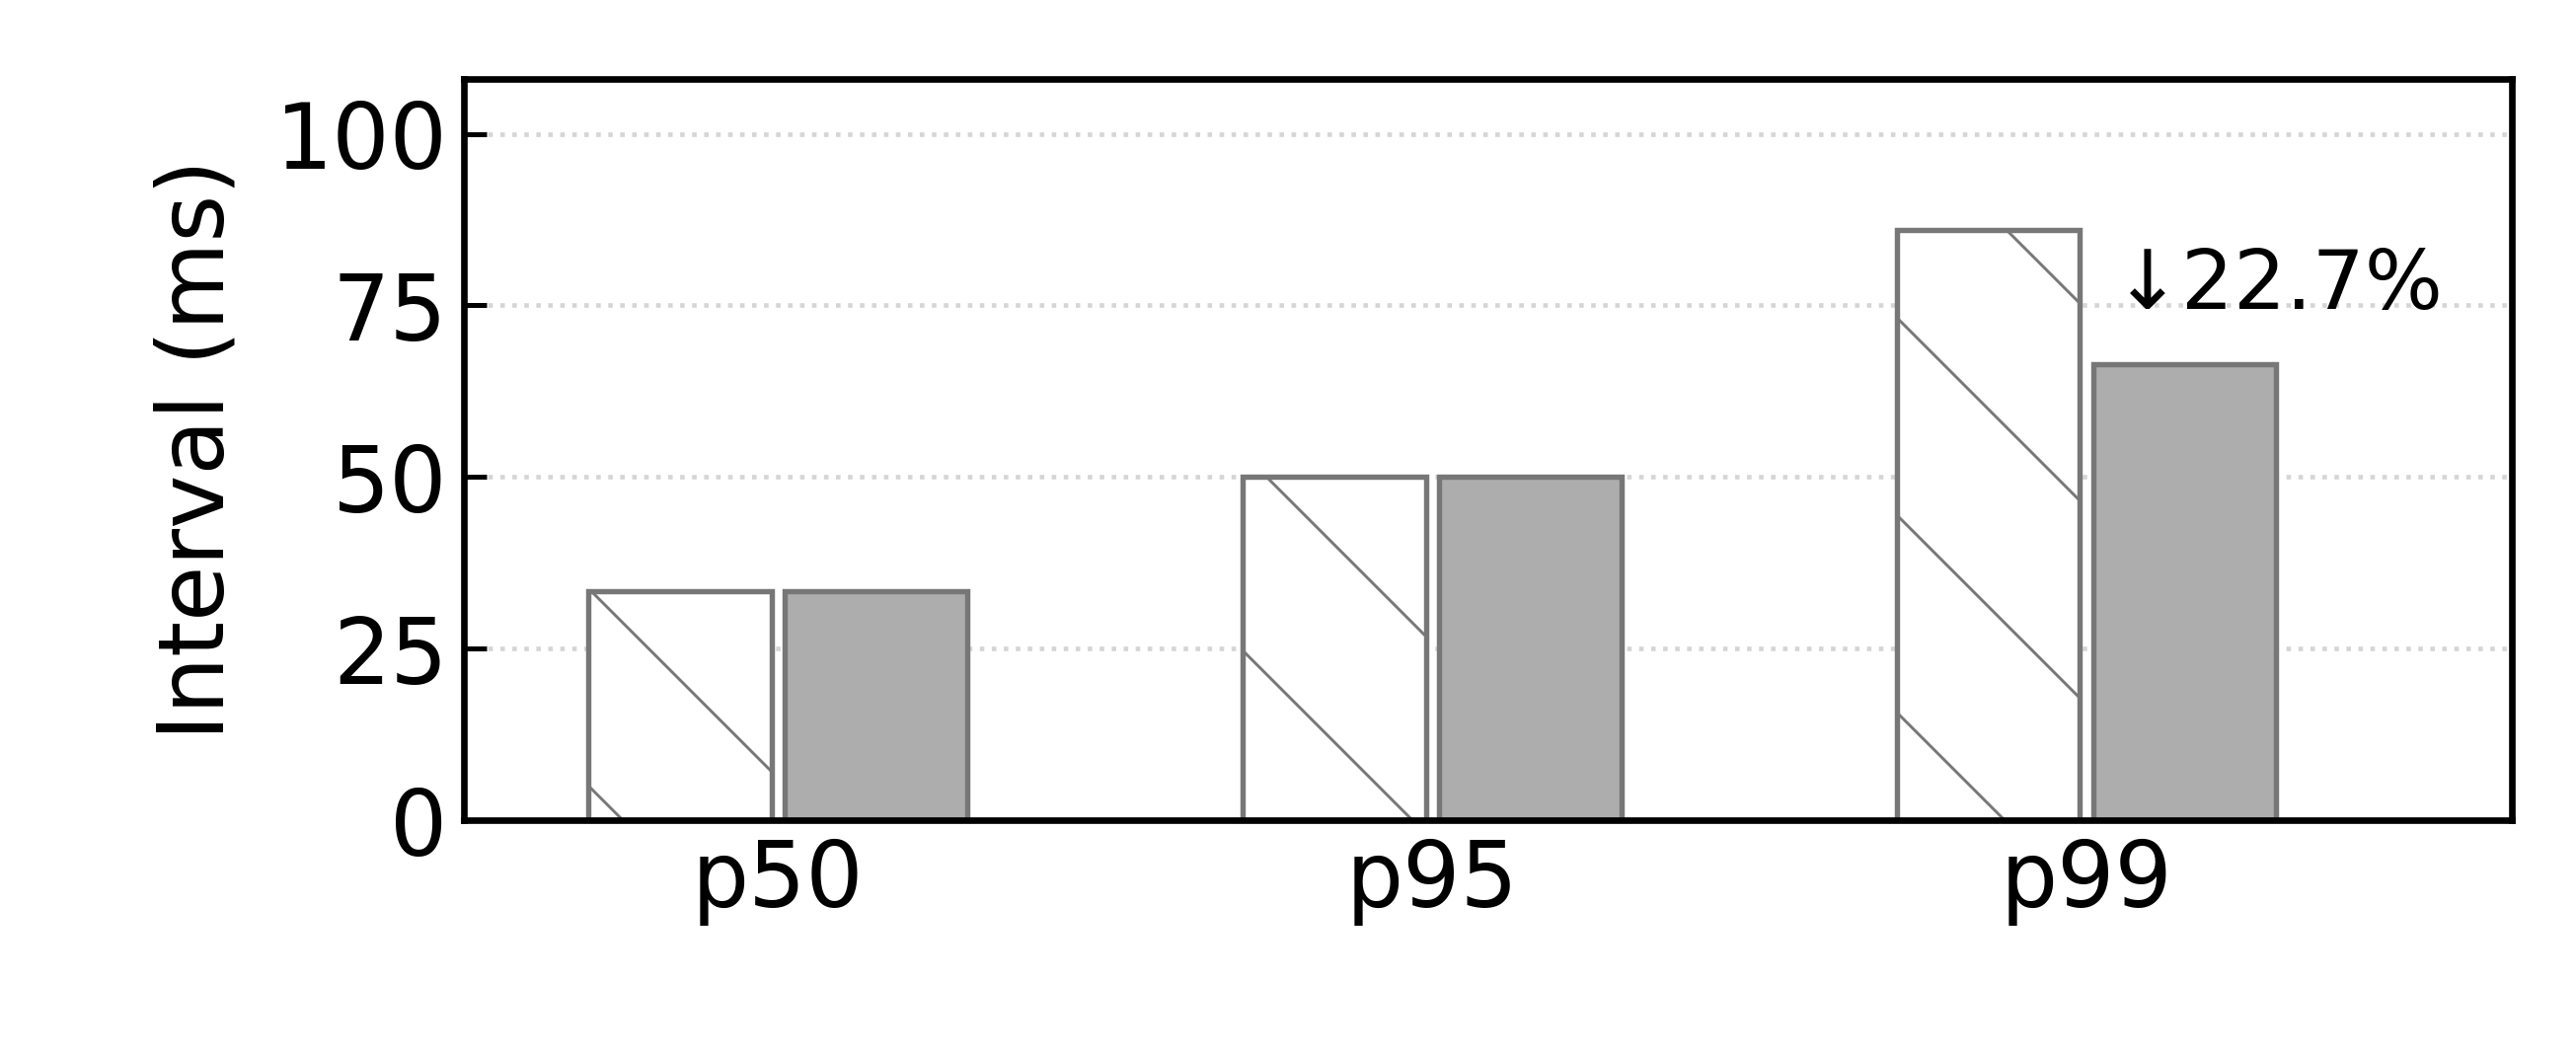
\includegraphics[width=\linewidth]{Figures/fig5_4_b_frame_interval.png}
    \subcaption{Frame Interval ($\downarrow$)}
    \label{fig:mindustry-interval}
  \end{subfigure}
  \caption{Mindustry 단독 실행에서 CFS와 RL-SchedExt의 게임 성능 비교. Frame Interval p50/p95/p99는 SurfaceFlinger의 게임 레이어 \texttt{present2present} 히스토그램을 기준으로 계산하였다.}
  \label{fig:mindustry-macro}
  \vspace{-0.7em}
\end{figure}

실험 결과, 두 Scheduler의 Frame Interval p50과 p95는 각각 33\,ms와 50\,ms로 동일하였으나, p99는 CFS의 86\,ms에서 RL-SchedExt의 66\,ms로 감소하여 23.3\% 감소하였다. 이는 일반적인 프레임 출력 간격은 유사하게 유지하면서도, 일부 프레임에서 발생하는 긴 출력 지연을 완화하였음을 보여준다.

종합하면, RL-SchedExt는 실제 Android Gaming Workload에서 Average FPS를 향상시키는 동시에 Frame Interval의 Tail Latency를 감소시켰다. 이러한 결과는 제안한 Scheduler가 게임의 전반적인 화면 갱신 성능뿐 아니라 간헐적인 화면 끊김(Stuttering)과 관련된 Frame Pacing 안정성도 개선할 수 있음을 보여준다.


\chapter{Conclusion}

\section{Conclusion}

In this work, we proposed a \emph{Memory Fabric} for multi-chiplet GPU systems with high-bandwidth memory (HBM). By exploiting otherwise unused shoreline on the HBM logic die, the proposed design uses die-to-die (D2D) interconnects to add memory-side paths, thereby expanding bisection bandwidth without requiring aggressive packaging assumptions. We further showed that direct memory-to-memory movement offloading, supported by a near-memory Data Movement Engine (DME), can reduce data movement overhead and alleviate contention on reticle-limited GPU-to-GPU links. Overall, the proposed memory fabric turns the HBM shoreline from a passive packaging constraint into an active architectural resource for improving path diversity, mitigating congestion, and accelerating communication-intensive GPU workloads.


% \section{Quantum Communication}

% There have been extensive studies on cognitive radio in recent years. To enhance the performance gain of original cognitive radio networks (CRNs), leveraging cooperative diversity has attracted a lot of attention \cite{SOCA1}...

% \subsection{Examples}


% \section{Applications of Quantum Communication}

% Despite its potential to improve the throughput, spatial domain diversity was not fully considered in the studies of original CCRNs. Utilizing the spatial domain for the communications, the concept of MIMO has been adopted in many cases to increase the wireless capacity \cite{EF1,FD2}...


% \chapter{Proposed Architecture and Its Application}

% \section{Proposed Architecture}

% Let us consider an MIMO-CCRN with one PL and one SL. Each PU has one legacy antenna and each SU has two STAR antennas. The duration of one communication time frame is divided into two phases \cite{RVP2,ML2} ...
%%
%% 표 삽입 예시
%% Example. how to insert table
%%
% \begin{table}[t]
% \caption[Enter the caption title here]{Energy stability $E$ (eV) per molecule of all meta-stable
% isomer states of C$_{60}$ opening process for forming the (5,5) cap.
% In the SW-I and SW-II, both ferromagnetic (Ferro) and paramagnetic (Para)
% spin configurations are obtained, whereas only non-magnetic configuration
% is obtained in the BF, SW-III, and CAP(5,5).
% $M$ is total magnetization $n_{\rm up}$-$n_{\rm down}$ in unit of $\mu_B$, where
% $n_{\rm up(down)}$ is the number of up (down) spins.
% }
% \label{mag-tab1}
% \begin{center}
% \begin{tabular} {ccccccccccc}
% \hline\hline
% & & BF &\multicolumn{2}{c}{SW-I}&&\multicolumn{2}{c}{SW-II}&SW-III&CAP&\\
% \cline{4-5} \cline{7-8}
% &               &   &  Para & Ferro &&   Para &  Ferro &      &      &\\
% \hline
% & $E$ (eV)      & 0 & 7.796 & 7.832 && 10.418 & 10.408 & 11.5 & 13.2 &\\
% & $M$ ($\mu_B$) & 0 &     0 &  1.94 &&      0 &   2.06 &    0 &    0 &\\
% \hline\hline
% \end{tabular}
% \end{center}
% \end{table}

%%
%% 그림 삽입 예시
%% Example. how to insert graph
%%
%% Note. 가급적 \includegraphics 명령을 사용하십시오.
%% Recommen : Use \includegraphics to insert graph.
%%
% \begin{figure}[t]
%     \centerline{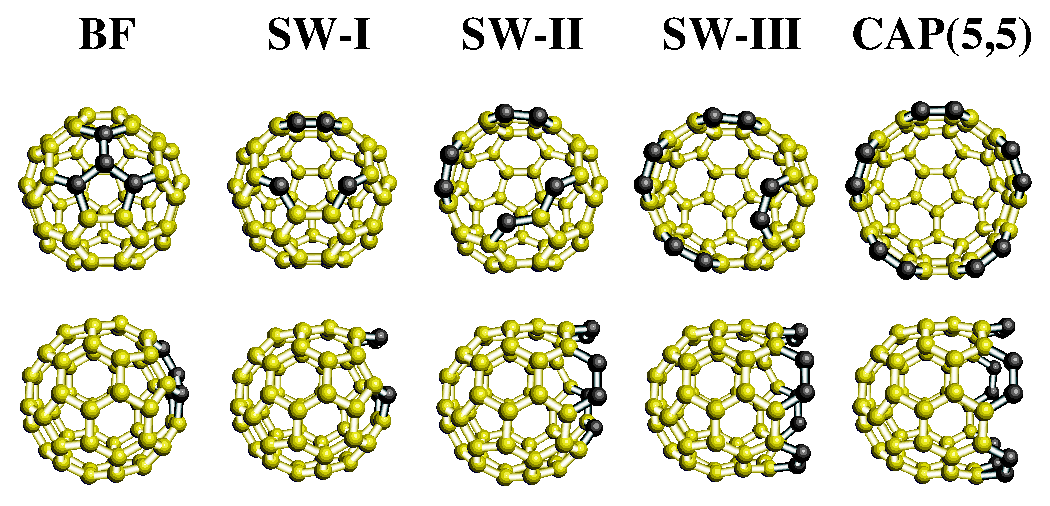
\includegraphics[width=12.5cm]{sample-fig1}}
%     \caption[Enter the caption title here]{ Ball-and-stick models of meta-stable isomers in
%         cage opening process from a C$_{60}$ buckminsterfullerene
%         to a (5,5) capsule. We name them BF and CAP(5,5).
%         Depending on the number of the Stone-Wales (SW) transformation,
%         we call the intermediate isomers with SW-I, SW-II, and SW-III.
%         Highlighted atoms are undercoordinated except BF.
%     } \label{mag-fig1}
% \end{figure}

% \section{Application}

% The achievable rates can be calculated by finding the statistics of the five signals transmitted that maximize the mutual information between $s_{t,XY}$ and $y_{t,XY}$ for $(X,Y)=(T,C), (C,N)$, and $(N,C)$ when $t=1$, and $(X,Y)=(C,R), (C,N)$, and $(N,C)$ when $t=2$ \cite{SOCA2,EF2}...


% \chapter{Concluding Remark}

% We have proposed a novel FD MIMO-CCRN framework providing a reasonable performance improvement compared with the conventional MIMO-CCRN framework...
%%
%% 참고문헌 시작
%% bibliography
%% It can be changed but should include sufficient information.

\bibliographystyle{IEEEtran}
\bibliography{reference}

% \begin{thebibliography}{00}

% \bibitem{FD1} 박상우, \underline{동시 송수신 안테나를 두 개 쓰는 협력 인지 무선통신망에 알맞은 전 이중 통신}, 한국과학기술원 석사 학위 논문, 2016.

% \bibitem{RVP1} 송익호, 박철훈, 김광순, 박소령, \underline{확률변수와 확률과정}, 자유아카데미, 2014.

% \bibitem{ML1} 송익호, 안태훈, 민황기, \underline{인지 무선에서의 광대역 주파수 검출 방법 및 장치}, 특허등록번호 10-1494966, 2015년 2월 12일.

% \bibitem{SOCA1} 호우위시, 이원주, 이승원, 안태훈, 이선영, 민황기, 송익호, “선형 판별 분석에서 부류안 분산 행렬의 영 공간 재공식화,” \underline{한국통신학회 2012년도 추계종합학술발표회}, 대한민국 고려대학교, 242-243쪽, 2012년 11월.

% \bibitem{EF1} 민황기, 안태훈, 이승원, 이성로, 송익호, “비간섭 전력 부하 감시용 고차 적률 특징을 갖는 전력 신호 인식,” \underline{한국통신학회논문지}, 제39C권, 제7호, 608-614쪽, 2014년 7월.



% \bibitem{FD2} S. Park, \textit{Full-Duplex Communication for Cooperative Cognitive Radio Networks with Two Simultaneous Transmit and Receive Antennas}, Master Thesis, Korea Adv. Inst. Science, Techn., Daejeon, Republic of Korea, 2016.

% \bibitem{RVP2}  I. Song, J. Bae, and S. Y. Kim, \textit{Advanced Theory of Signal Detection: Weak Signal Detection in Generalized Observations}, Springer-Verlag, 2002.

% \bibitem{ML2} I. Song, T. An, and J. Oh, \textit{Near ML decoding method based on metric-first search and branch length threshold,} registration no. US 8018828 B2, Sep. 13, 2011, USA. 

% \bibitem{SOCA2} H.-K. Min, T. An, S. Lee, and I. Song, “Non-intrusive appliance load monitoring with feature extraction from higher order moments,” in \textit{Proc. 6th IEEE Int. Conf. Service Oriented Computing, Appl.,} Kauai, HI, USA, pp. 348-350, Dec. 2013.

% \bibitem{EF2} I. Song and S. Lee, “Explicit formulae for product moments of multivariate Gaussian random variables,” \textit{Statistics, Probability Lett.,} vol. 100, pp. 27-34, May 2015.


% \end{thebibliography}



%%
%% 감사의 글 시작
%% Acknowledgement
%%
% @command acknowledgement 감사의글
% @options [1 | 2 | 3 |4 ]
% - 1 : 본문과 감사의 글이 둘 다 한글일 때  | 2 : 본문은 한글인데 감사의 글이 영어일 때 | 3 :  본문과 감사의 글이 둘 다 영어일 때  | 4 : 본문은 영어인데 감사의 글이 % 한글일 때 
%% It is optional.

% \acknowledgment[4]

% %%
% %% 약력 시작
% %% Curriculum Vitae
% %%
% % @command curriculumvitae 이력서
% % @options [1 | 2 | 3 |4 ]
% % - 1 : 본문과 약력이 둘 다 한글일 때  | 2 : 본문은 한글인데 약력이 영어일 때 | 3 :  본문과 약력이 둘 다 영어일 때  | 4 : 본문은 영어인데 약력이 한글일 때 
% %% It is optional and you can change form of this in the class file if you want.
% \curriculumvitae[4]

%     % @environment personaldata 개인정보
%     % @command     name         이름
%     %              dateofbirth  생년월일
%     %              birthplace   출생지
%     %              domicile     본적지
%     %              address      주소지
%     %              email        E-mail 주소
%     % - 위 6개의 기본 필드 중에 이력서에 적고 싶은 정보를 입력
%     % input data only you want
%     \begin{personaldata}
%         \name       {안 효 원}
%         \dateofbirth{1986}{01}{30}
%         \birthplace {대한민국 서울}
%         \address    {경기도 수원시 영통구 덕영대로 1462-14}
%     \end{personaldata}

%     % @environment education 학력
%     % @options [default: (none)] - 수학기간을 입력
%     \begin{education}
%         \item[2001. 3.\ --\ 2004. 2.] 속초고등학교
%         \item[2004. 2.\ --\ 2012. 8.] 고려대학교 전기전자전파공학부 (학사)        
%         \item[2025. 3.\ --\ 2026. 8.] 한국과학기술원 시스템아키텍트대학원 (석사)
%     \end{education}

%     % @environment career 경력
%     % @options [default: (none)] - 해당기간을 입력
%     \begin{career}
%         \item[2012. 7.\ --\ 2025. 2.] 삼성전자        
%     \end{career}

%     % @environment activity 학회활동
%     % @options [default: (none)] - 활동내용을 입력
% %%    \begin{activity}
% %%        \item J. Choi, \textbf{Yong-Hyun Kim}, K.J. Chang, and D. Tomanek,
% %%             \textit{Occurrence of itinerant ferromagnetism in C/BN superlattice
% %%             nanotubes}, 5th Asian Workshop on First-Principles Electronic
% %%             Structure Calculations, Seoul (Korea), October., 2002.
% %%    \end{activity}

%     % @environment publication 연구업적
%     % @options [default: (none)] - 출판내용을 입력
% %     \begin{publication}
% %         %\item \textbf{Yong-Hyun Kim}, J. Choi, K.J. Chang, and D. Tomanek,
% %         %     \textit{Magnetic instability in partly opened C$_{60}$ isomers},
% %         %     in preparation.
% %         \item {\bf 안효원}, 이재원, 하승수, 박진우, 이현이, 정지영,
% % ``이종 칩렛 시스템을 위한 강화학습 기반 메모리 중심 배치 및 라우팅 최적화,"
% % \textit{대한전자공학회 하계종합학술대회}, 2026 (to be published).
% %         \item {하승수*, \bf 안효원}*,
% % ``SPHBM 기반 메모리 대역폭 및 용량 확장 패키지 구조,"
% % \textit{대한전자공학회 하계종합학술대회}, 2026 (to be published).
% %         \item Junho Park, {\bf Hyowon An}, Haeseok Suh, Youngsu Yoon, Hyuni Lee and Joungho Kim,
% % ``HBM-HBF-Centric Memory Pooling Architecture with Custom Base Die for Terabyte-Scale LLM Inference," in 
% % \textit{IEEE Computer Architecture Letters (CAL)}, 2026 (to be published).
% %         \item Hyuni Lee, Haeyeon Kim, JungHyun Lee, Inyoung Choi, Jaehun Lee, {\bf Hyowon An}, Chaemin Yang, and Joungho Kim,
% % ``Mem-Village: A Hybrid HBF-HBM Architecture on Glass for Ultra-Scale AI Inference Systems," in 
% % \textit{2025 IEEE Electrical Design of Advanced Packaging and Systems (EDAPS)}, 2025, pp. 1-3.
% % \end{publication}

  \label{paperlastpagelabel}     % <-- 추가 부분: 마지막 페이지 위치 지정	
%% 본문 끝
\end{document}
